\def\splashfigure#1{
    \begin{figure*}[#1]
        \centering
        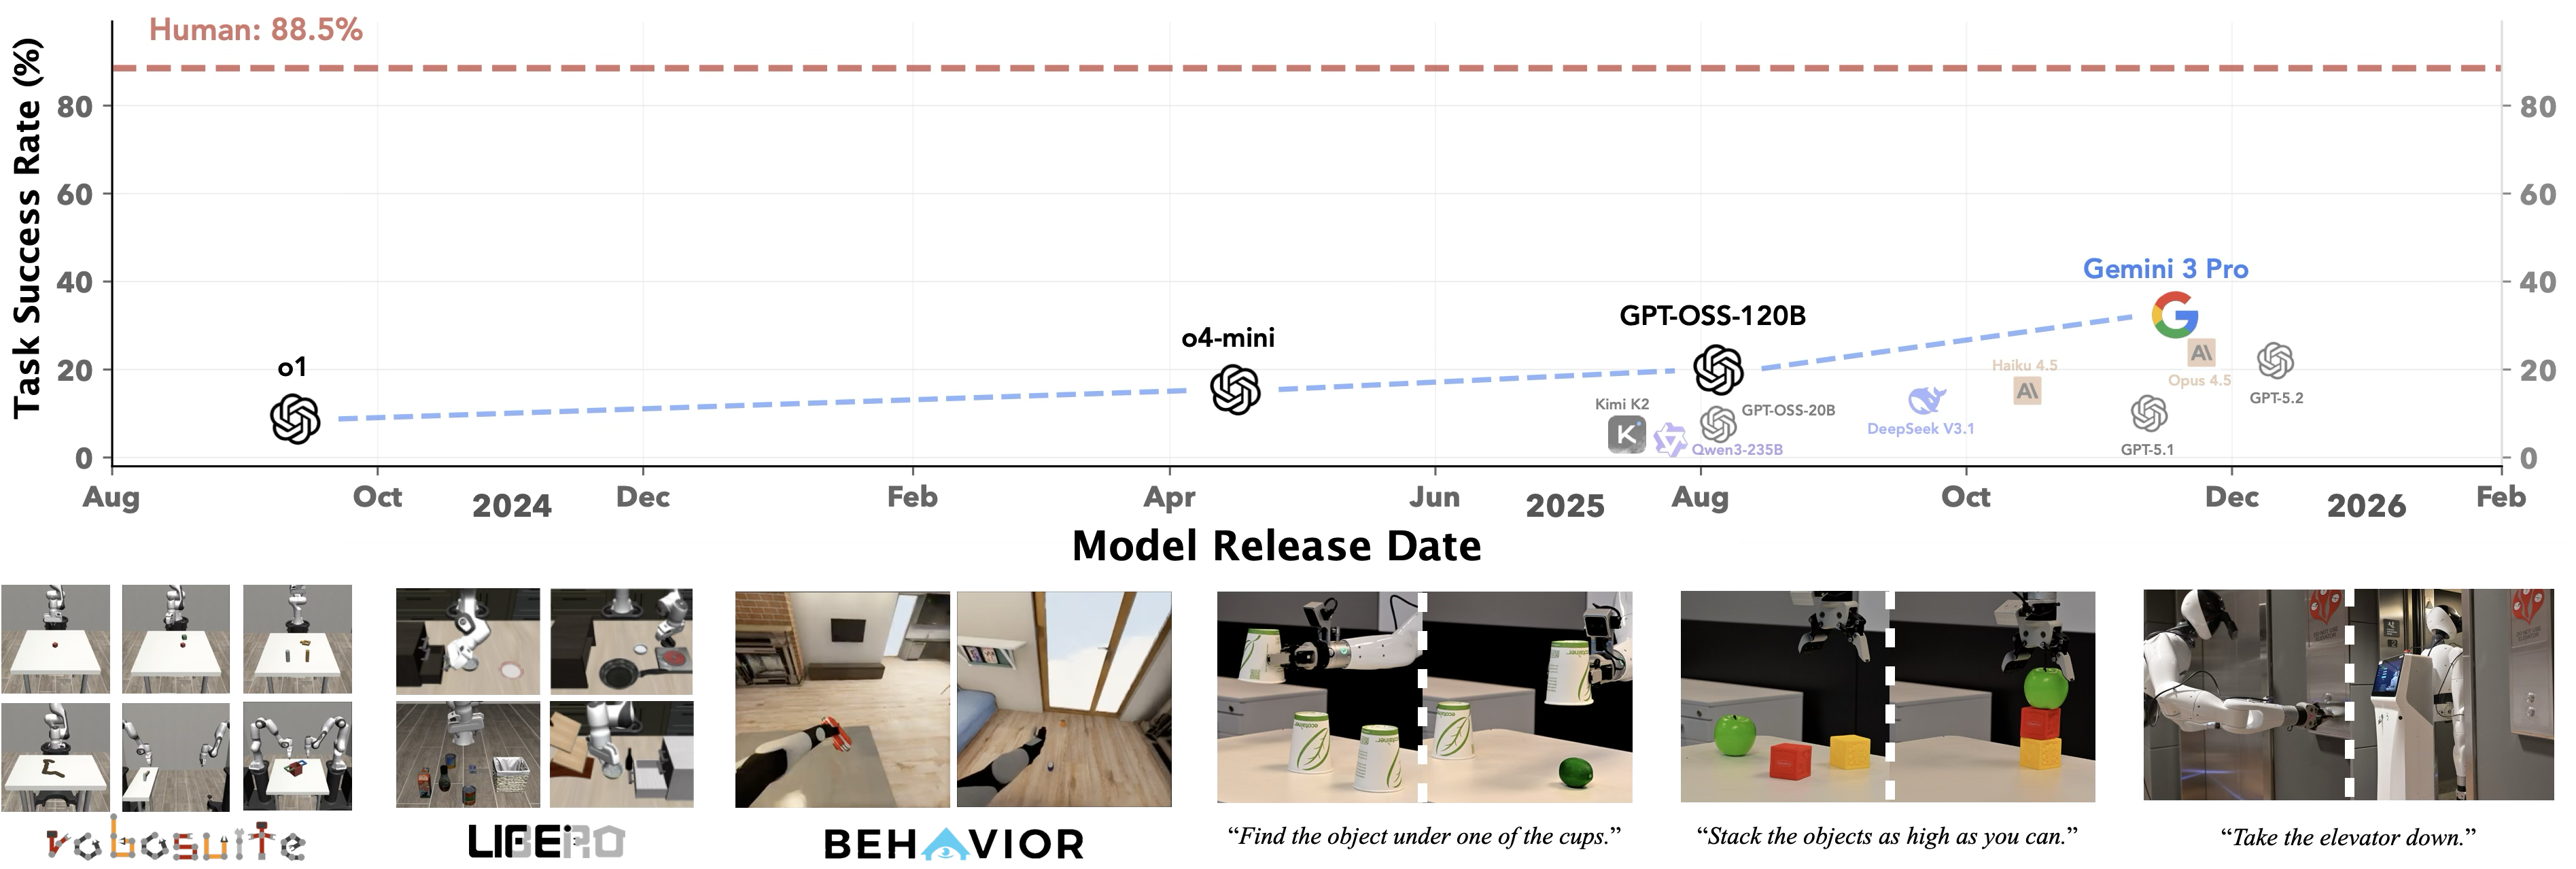
\includegraphics[width=\textwidth]{assets/figures/splash_figure_v3.png}
        \caption{
        \textbf{(Top)} CaP-Bench Task Success Rate over Model Release Date: across 7 tasks and 12 models, we compare the success rates of model-generated robot-control programs against those of human expert-written programs. We find that while (vision-) language models have achieved capabilities comparable to humans in other domains~\cite{jimenez2024swebench, rein2024gpqa, hendrycks2020mmlu}, they still trail behind human performance in writing code that controls robots for manipulation tasks. \textbf{(Bottom)}: \gymname{} integrates Robosuite~\cite{zhu2020robosuite}, LIBERO-PRO~\cite{zhou2025liberopro}, and BEHAVIOR~\cite{li2024behavior1k}. We further present \sysname{} (\cref{sec:capagent}), a training-free agentic framework that recovers near human-level performance on several manipulation tasks and achieves success rates comparable to—and in some cases exceeding—those of post-trained VLAs, without any task-specific training data.
        }
        \label{fig:splash_fig}
    \end{figure*}
}

\def\capgymenvfigure#1{
    \begin{figure*}[#1]
        \centering
        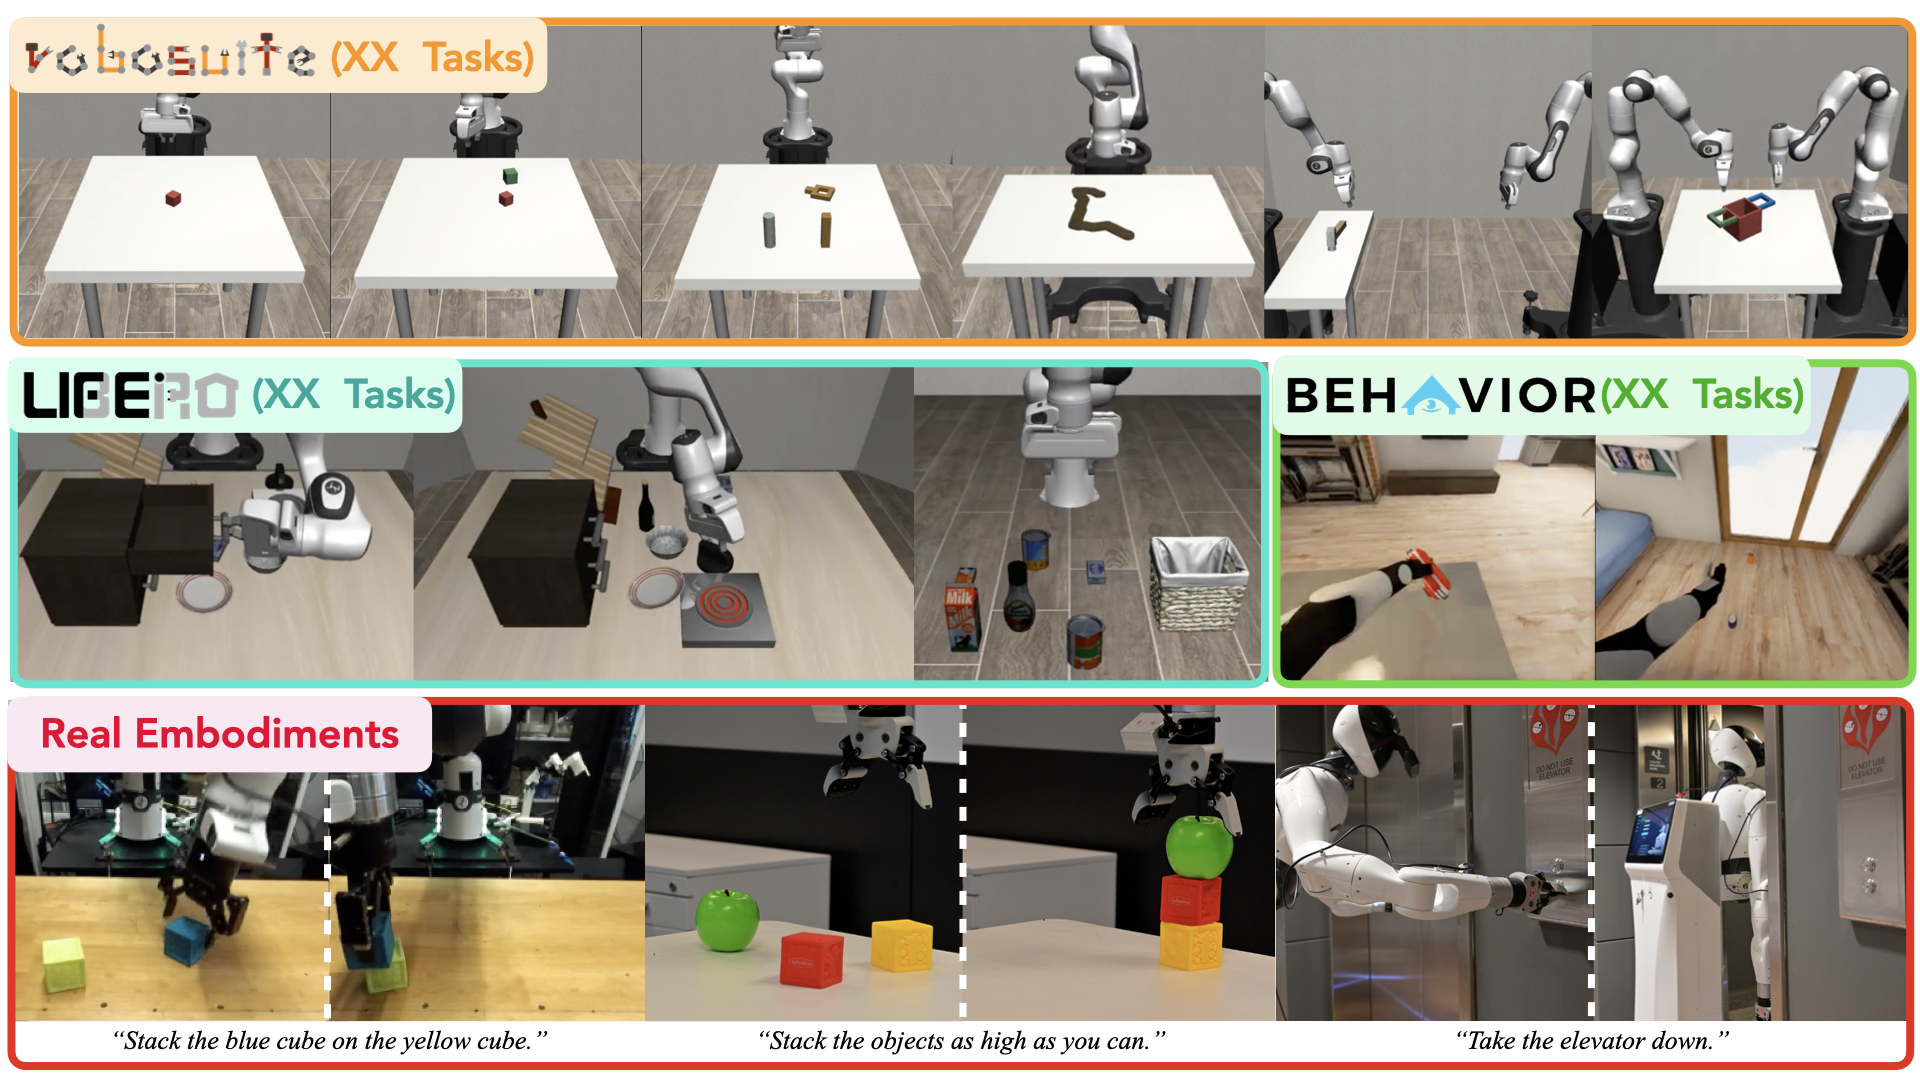
\includegraphics[width=\textwidth]{assets/figures/capgym_envs_fig.png}
        \caption{
        \textbf{(Top and Middle Row) \gymname{} environments.}
        \gymname{} integrates XX tasks from RoboSuite~\cite{zhu2020robosuite}, LIBERO-PRO~\cite{zhou2025liberopro}, and BEHAVIOR~\cite{li2024behavior1k}. \textbf{(Bottom Row) CaP-Agent0 in real-world manipulation.} We deploy \sysname{} on a real-world AgiBot G1~\cite{bu2025agibot_iros} robot to perform a wide variety of robot manipulation tasks zero-shot (see Appendix \cref{app:real-world-agibot}).
        }
        \label{fig:capgym_envs}
    \end{figure*}
}

\def\capagentfigure#1{
    \begin{figure*}[#1]
        \centering
        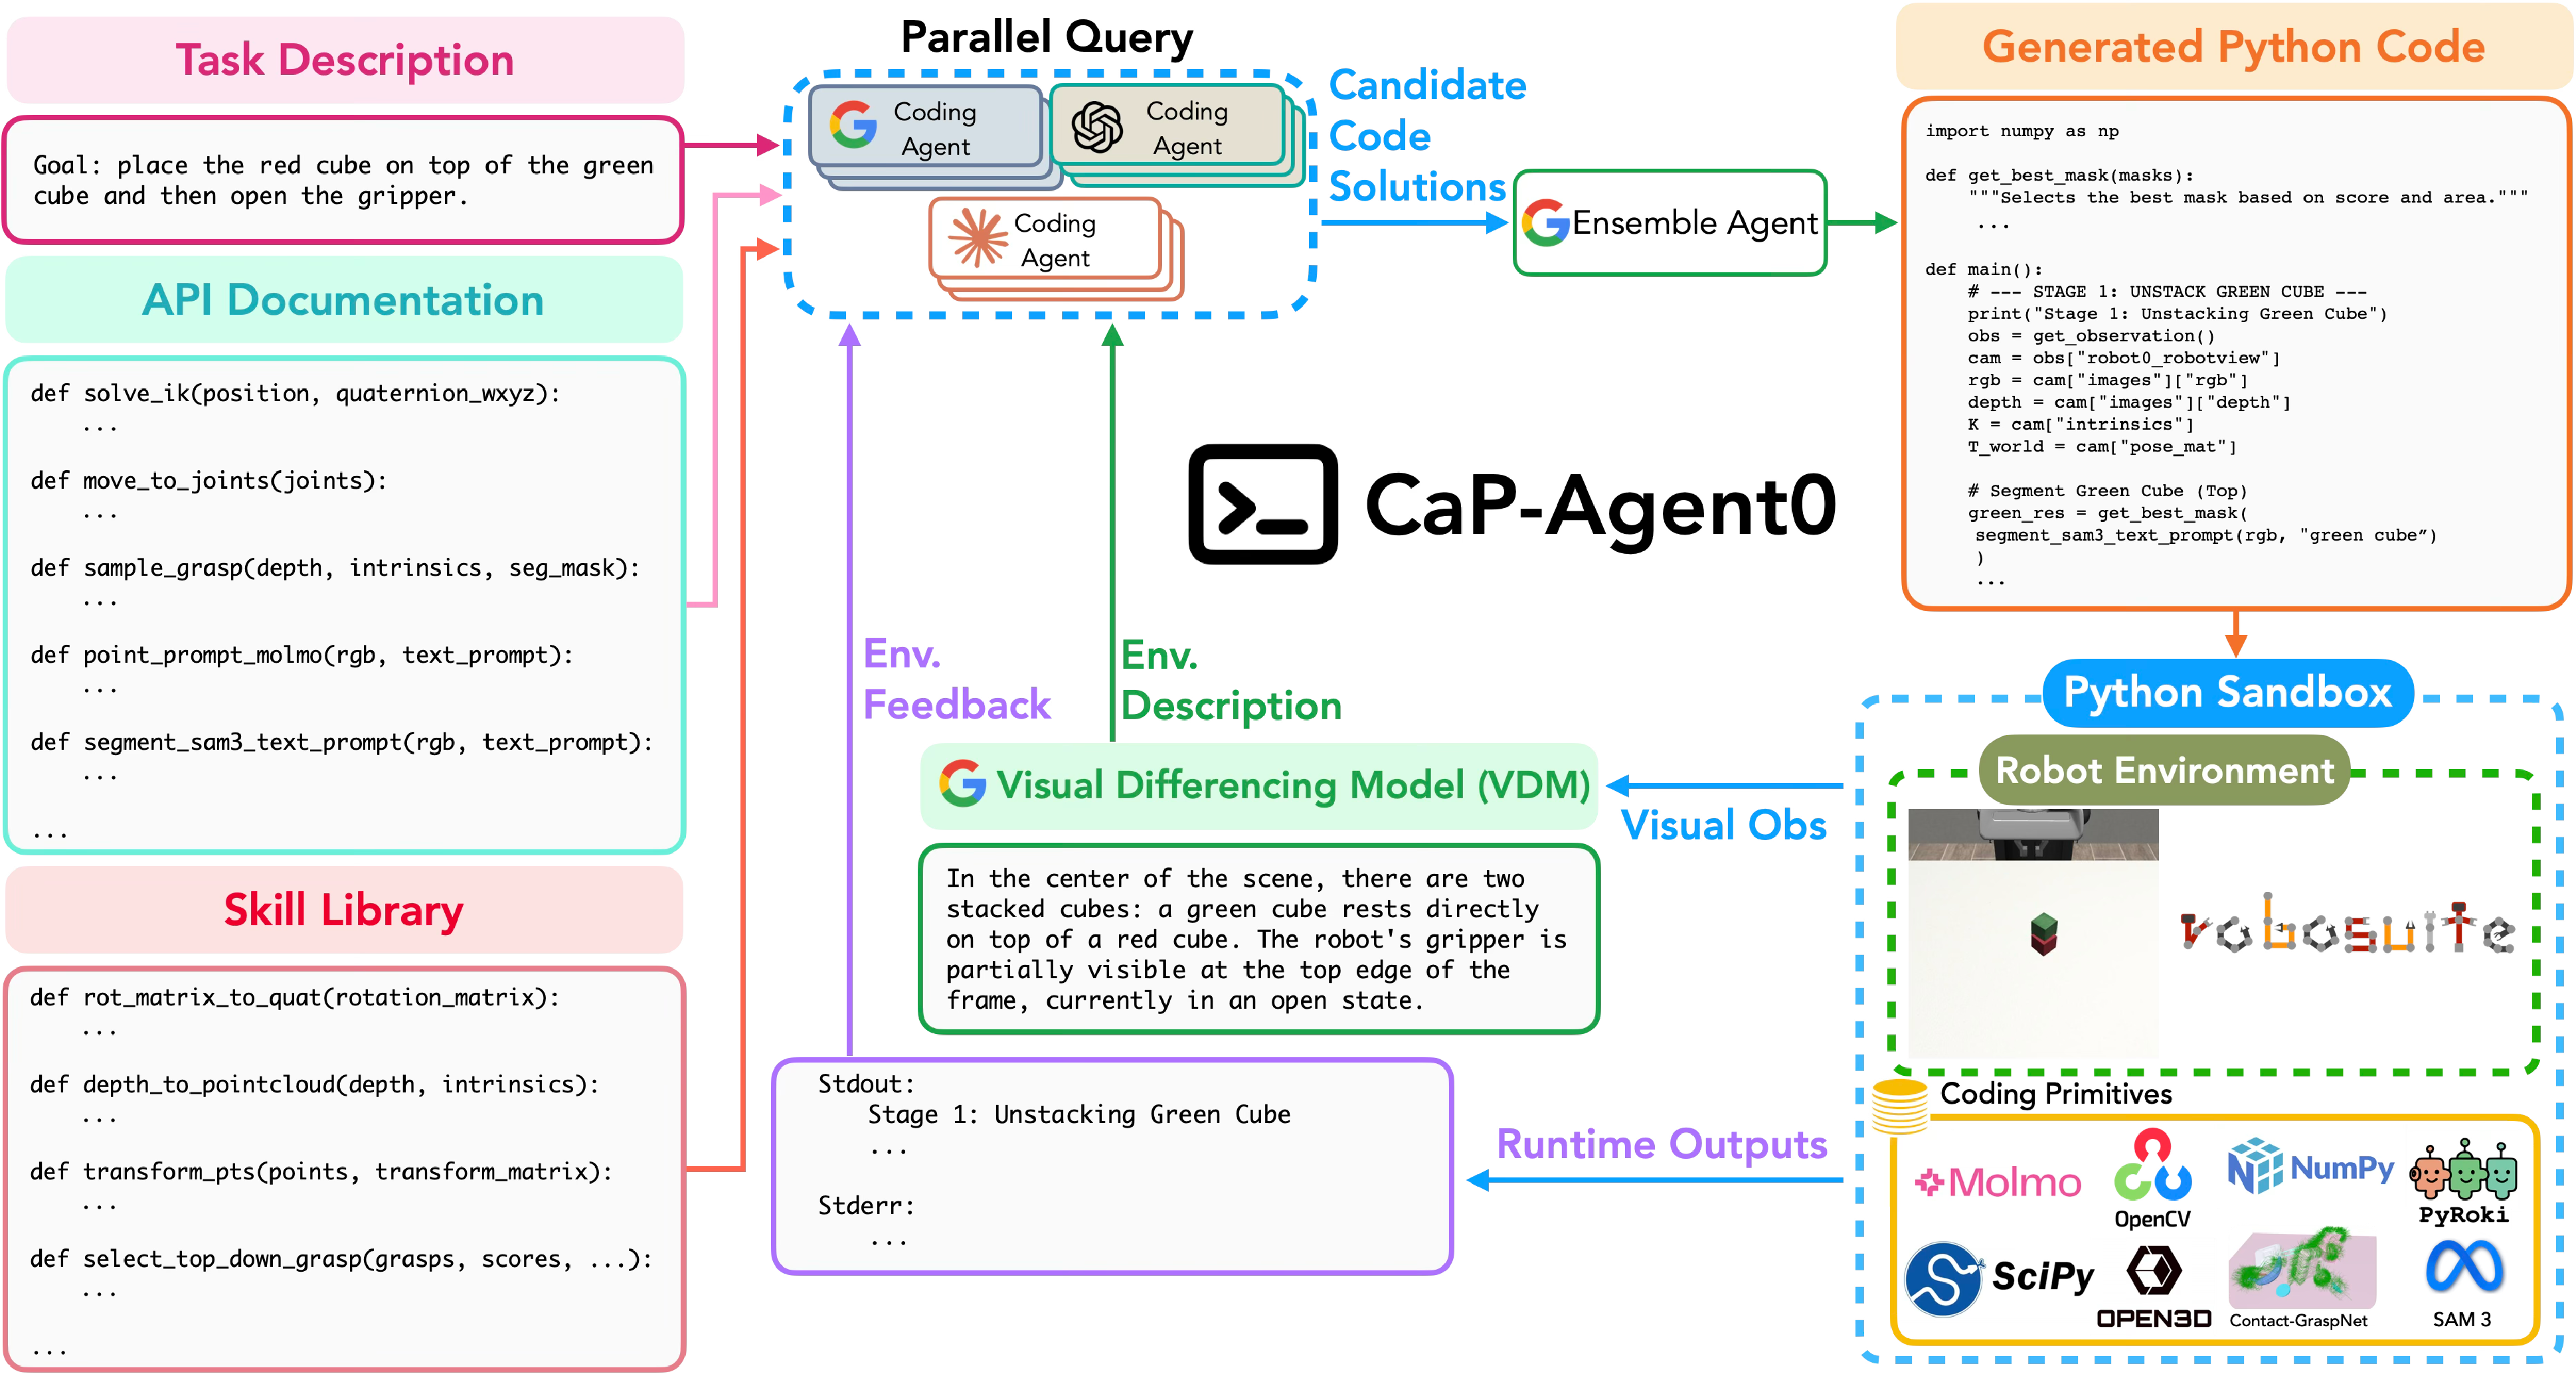
\includegraphics[width=\textwidth]{assets/figures/capagent0_figure.pdf}
        \caption{
        \textbf{CaP-Agent0.} CaP-Agent0 incorporates an auto-synthesized skill library of auxiliary utility generated by coding agents during CaP-Bench, a visual differencing model (VDM) which provides a textual description of the initial scene and for each subsequent turn what changes have occurred in the scene since, and a parallel reasoning system where multiple coding agents are provided the same prompt. These coding agents then generate candidate code solutions that may solve the task and the ensemble agent must then synthesize these code generations into a final code snippet which is then executed in the Python sandbox containing the robot environment, whether that environment may be a simulator like Robosuite or on a real robot. For more details see Section \ref{sec:capagent}.
        }
        \label{fig:capagent0_sys}
    \end{figure*}
}

\def\abstractionlevelfigure#1{
    \begin{figure*}[#1]
        \centering
        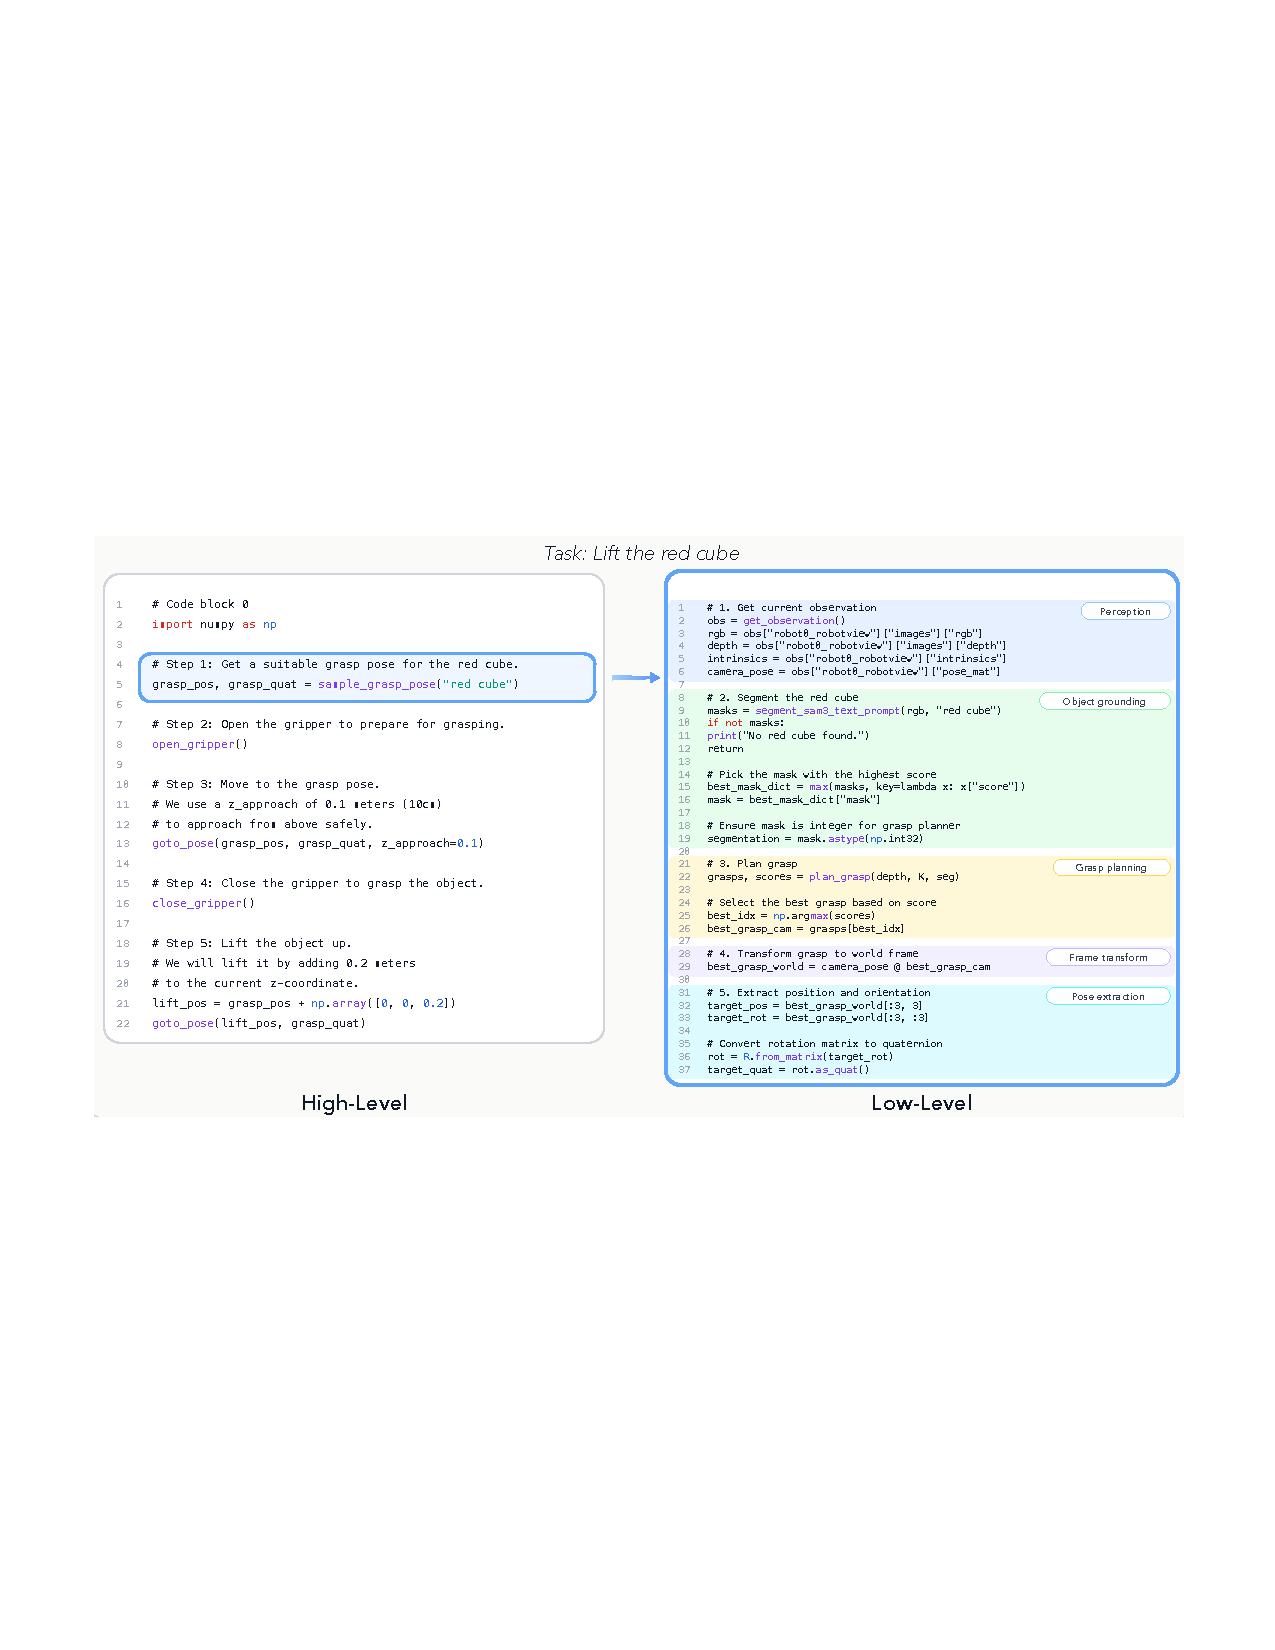
\includegraphics[width=\textwidth]{assets/figures/high_vs_low.pdf}
        \caption{
        \textbf{(Left)} An example of code generated by Gemini-3-Pro for completing the task \textit{``lift the red cube"} using the high-level primitives. \textbf{(Right)} Code generated by Gemini-3-Pro using just low-level primitives to achieve the same functionality as a single high-level primitive. For more details on the differences between high and low-level primitives, see Section \ref{subsec:singleturn} and Appendix \ref{app:apis}.
        }
        \label{fig:abstractionlevel_diff}
    \end{figure*}
}

\def\humanvsmodels#1{
    \begin{figure*}[#1]
        \centering
        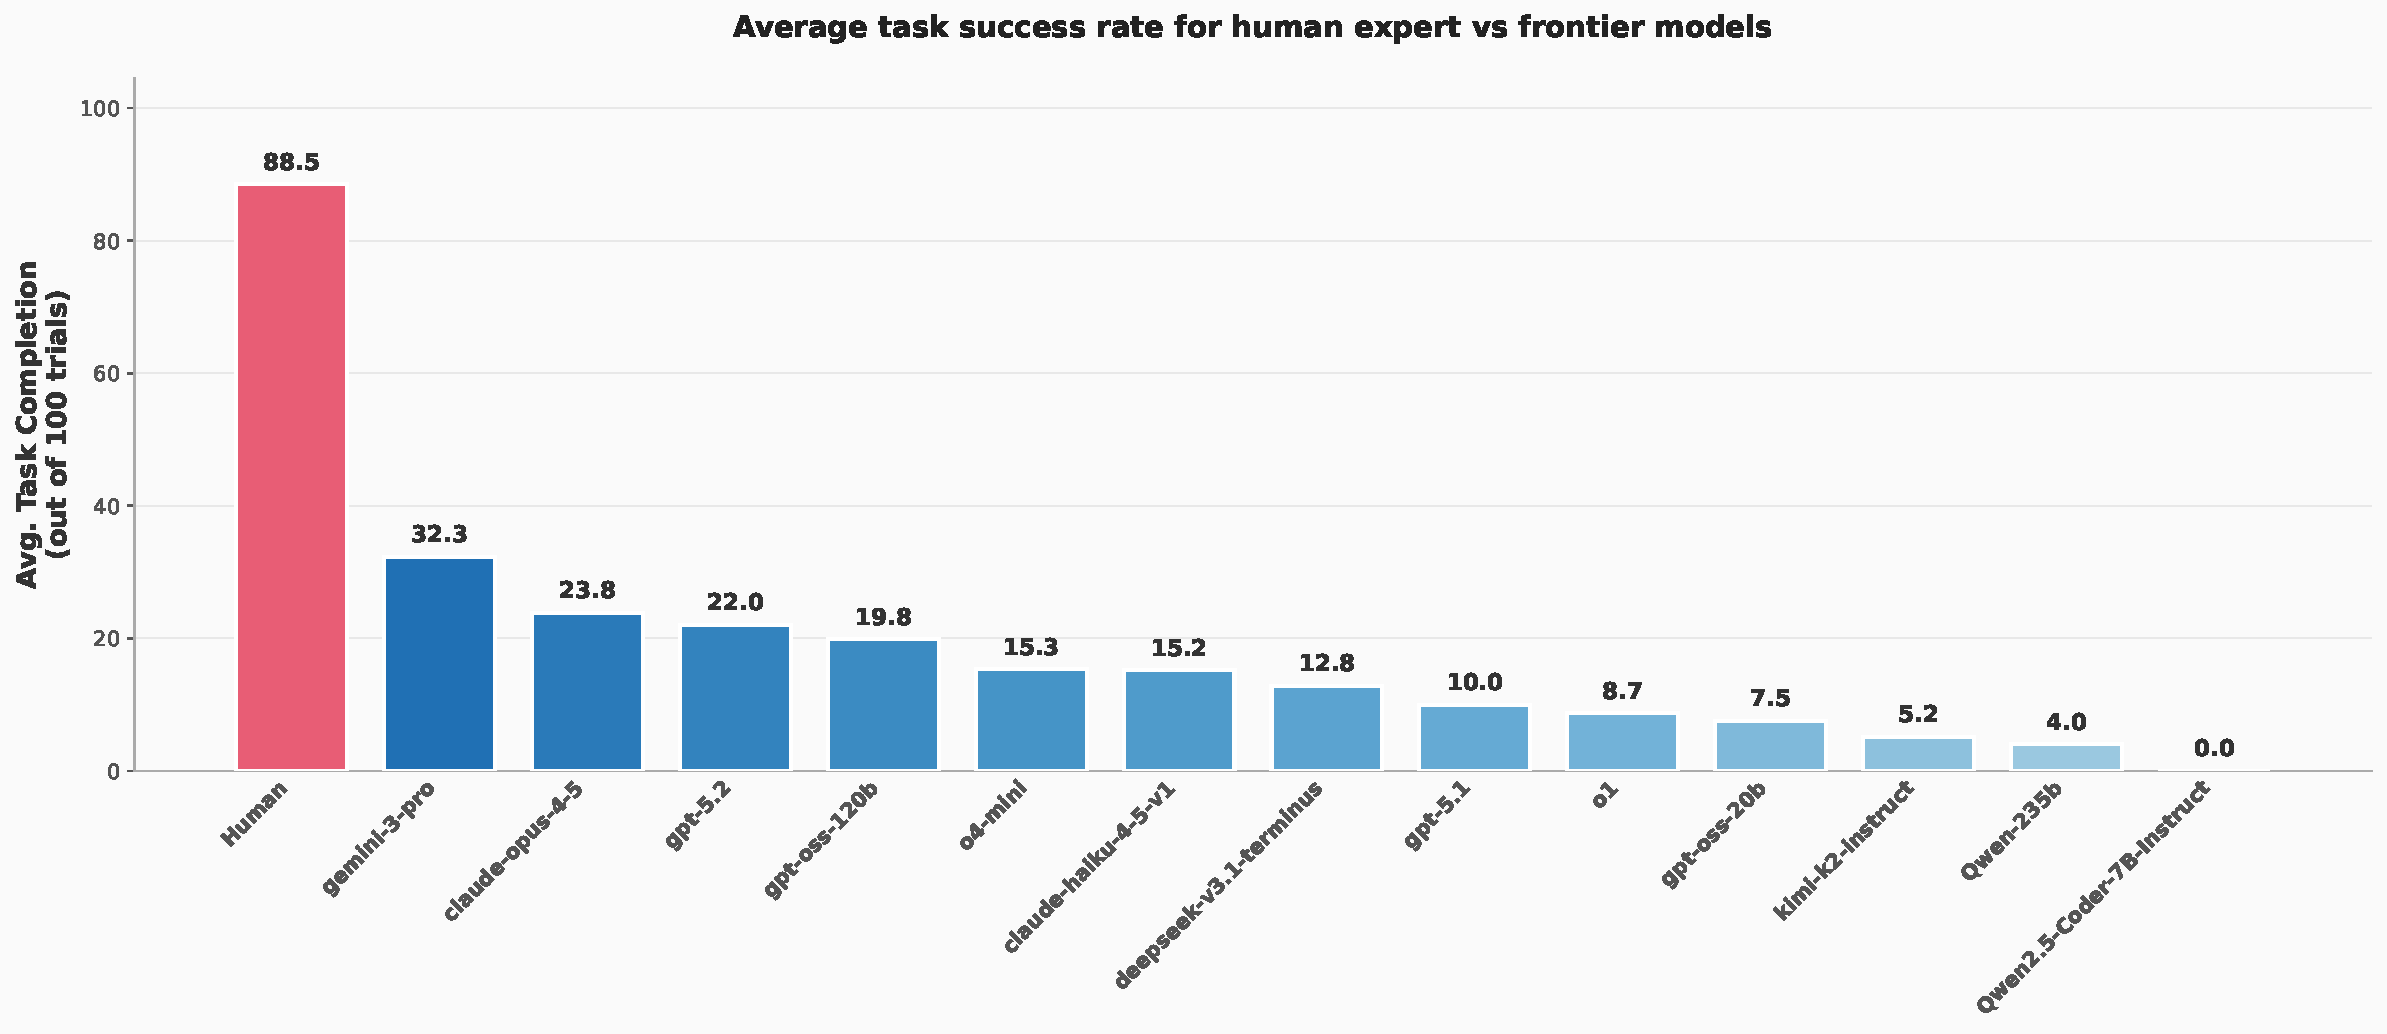
\includegraphics[width=\textwidth]{assets/figures/human_vs_single_turn.pdf}
        \caption{Performance comparison between human experts and frontier models on abstraction tier S4.}
        \label{fig:human_vs_single_turn}
    \end{figure*}
}

\def\abstractionincrease#1{
    \begin{figure}[#1]
        \centering
        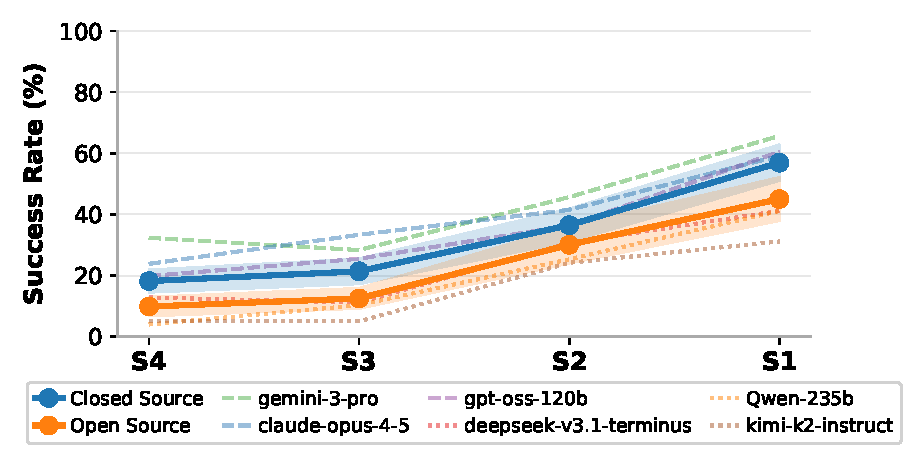
\includegraphics[width=0.45\textwidth]{assets/figures/abstraction_analysis.pdf}
        \caption{Average task success rate across open-source and closed-source models as primitive abstraction increases. As primitive abstraction increases S4 (per model performance illustrated in \cref{fig:splash_fig}) to S1 (high level primitives with full state observation), the success rate increases. This can only in part be attributed to reduced code correctness at S3-S4, see \cref{fig:codecompilation}.}
        \label{fig:abstraction_increase}
    \end{figure}
}

\def\codecompilation#1{
    \begin{figure}[#1]
        \centering
        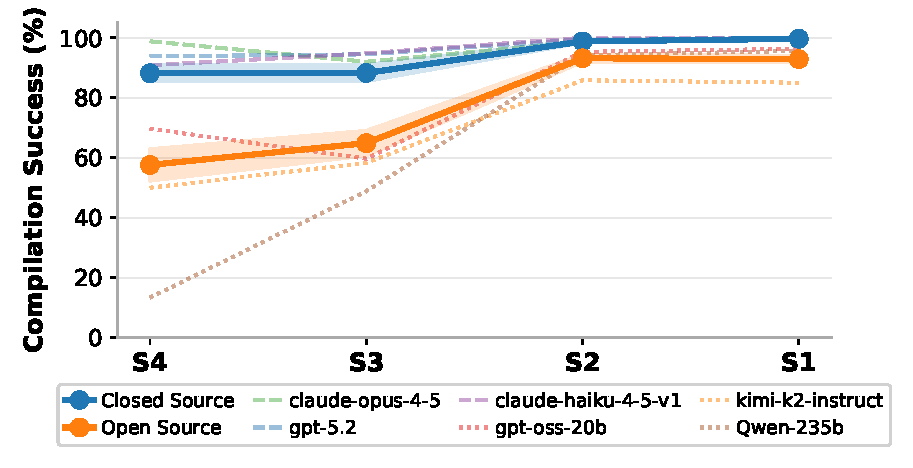
\includegraphics[width=0.45\textwidth]{assets/figures/compilation_analysis.pdf}
        \caption{Code Execution Success Rate vs primitive abstraction.}
        \label{fig:codecompilation}
    \end{figure}
}

\def\iclapiusage#1{
    \begin{figure}[#1]
        \centering
        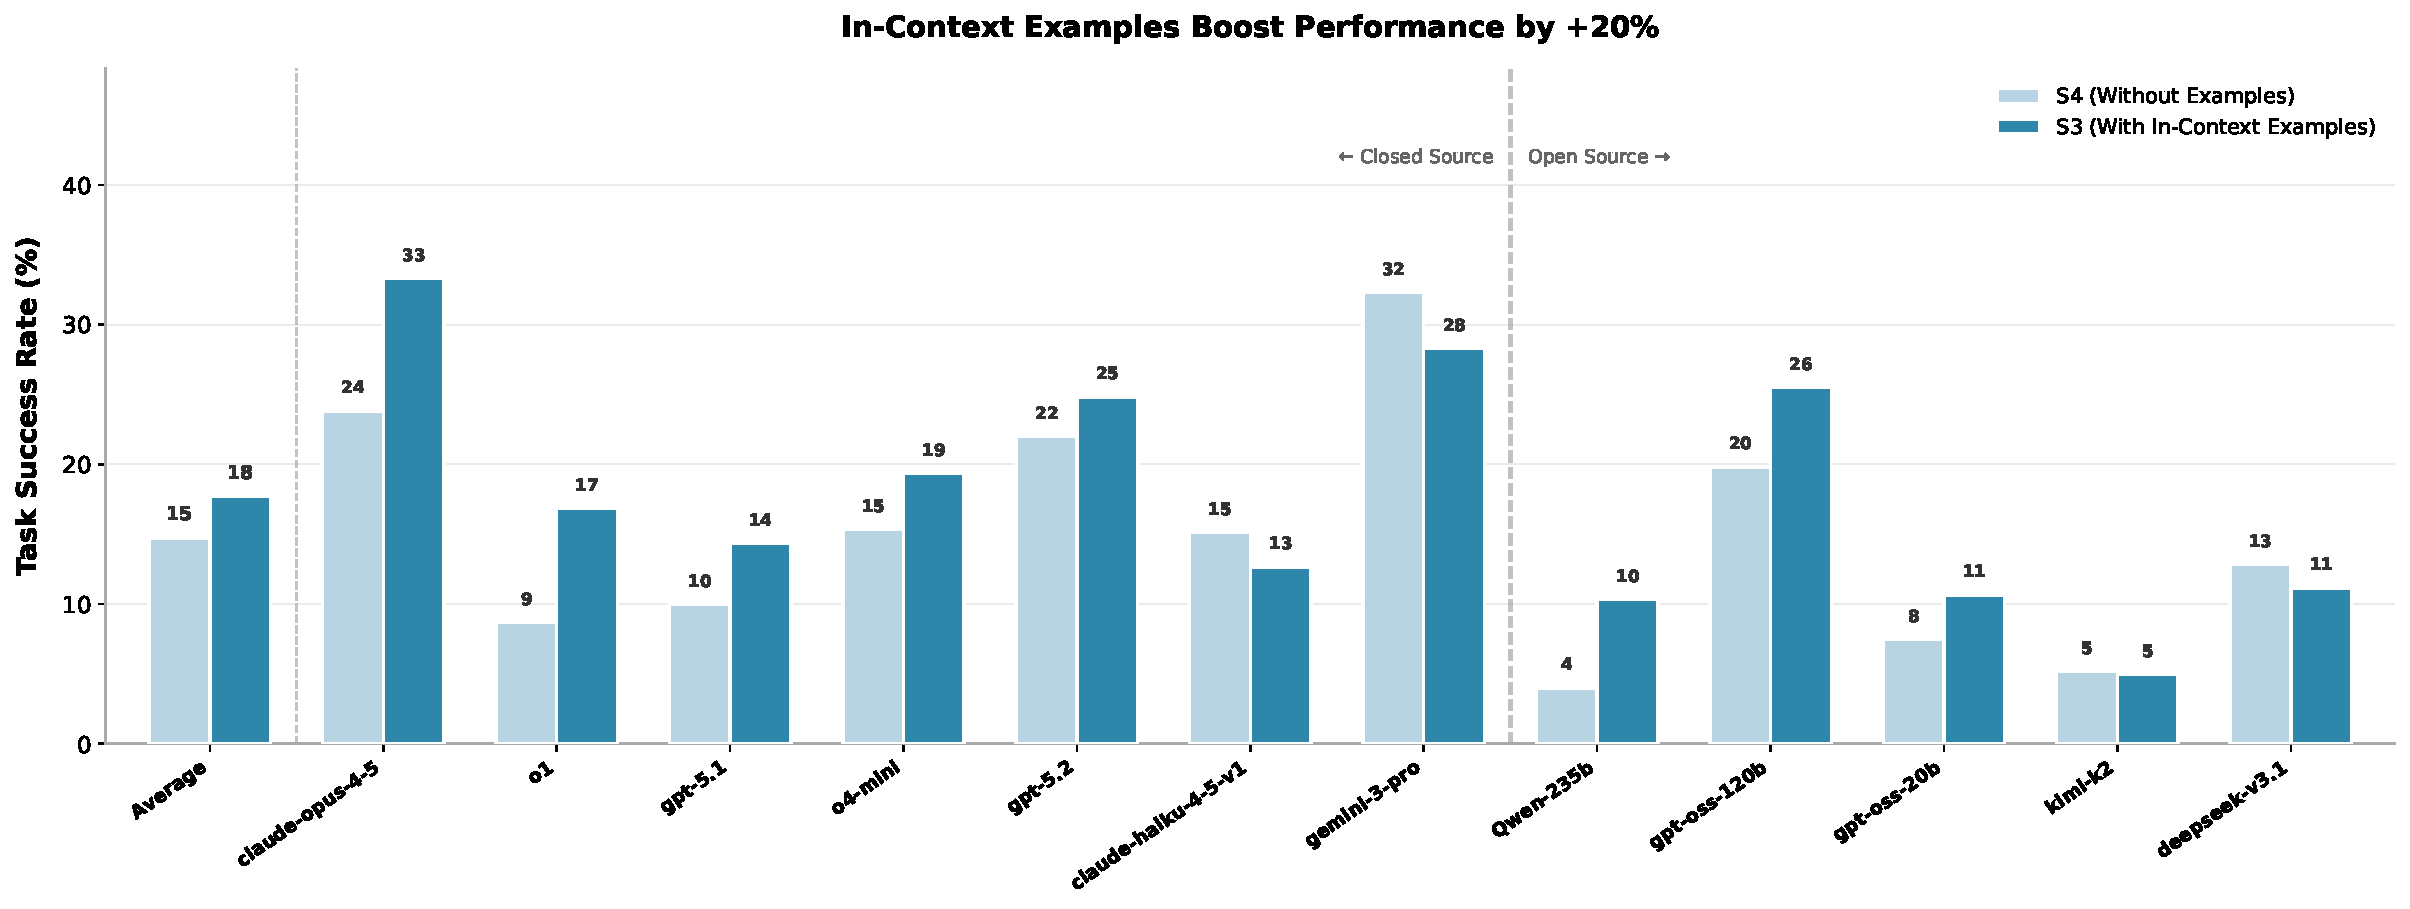
\includegraphics[width=\textwidth]{assets/figures/incontext_examples_comparison.pdf}
        \caption{Per-model breakdown of usefulness of in-context API Usage}
        \label{fig:iclapiusage}
    \end{figure}
}

\def\pertaskicl#1{
    \begin{figure}[#1]
        \centering
        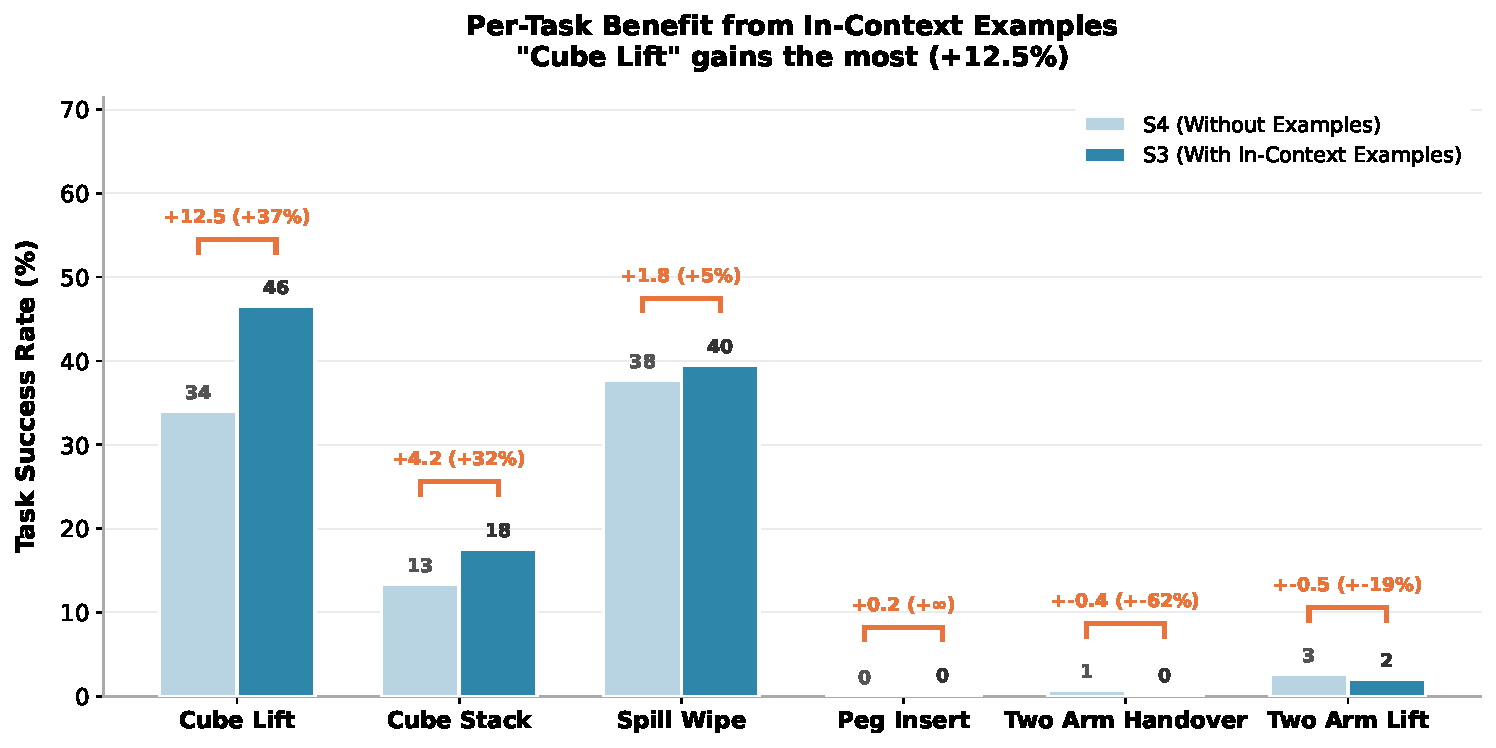
\includegraphics[width=\textwidth]{assets/figures/incontext_per_task_improvement.pdf}
        \caption{Average model performance improvement from In-Context API Usage Examples. The ``Cube Lift" task across all models sees an improvement of 12.5\% improvement in success rate.}
        \label{fig:pertaskicl}
    \end{figure}
}

\def\multiturnvssingle#1{
    \begin{figure}[#1]
        \centering
        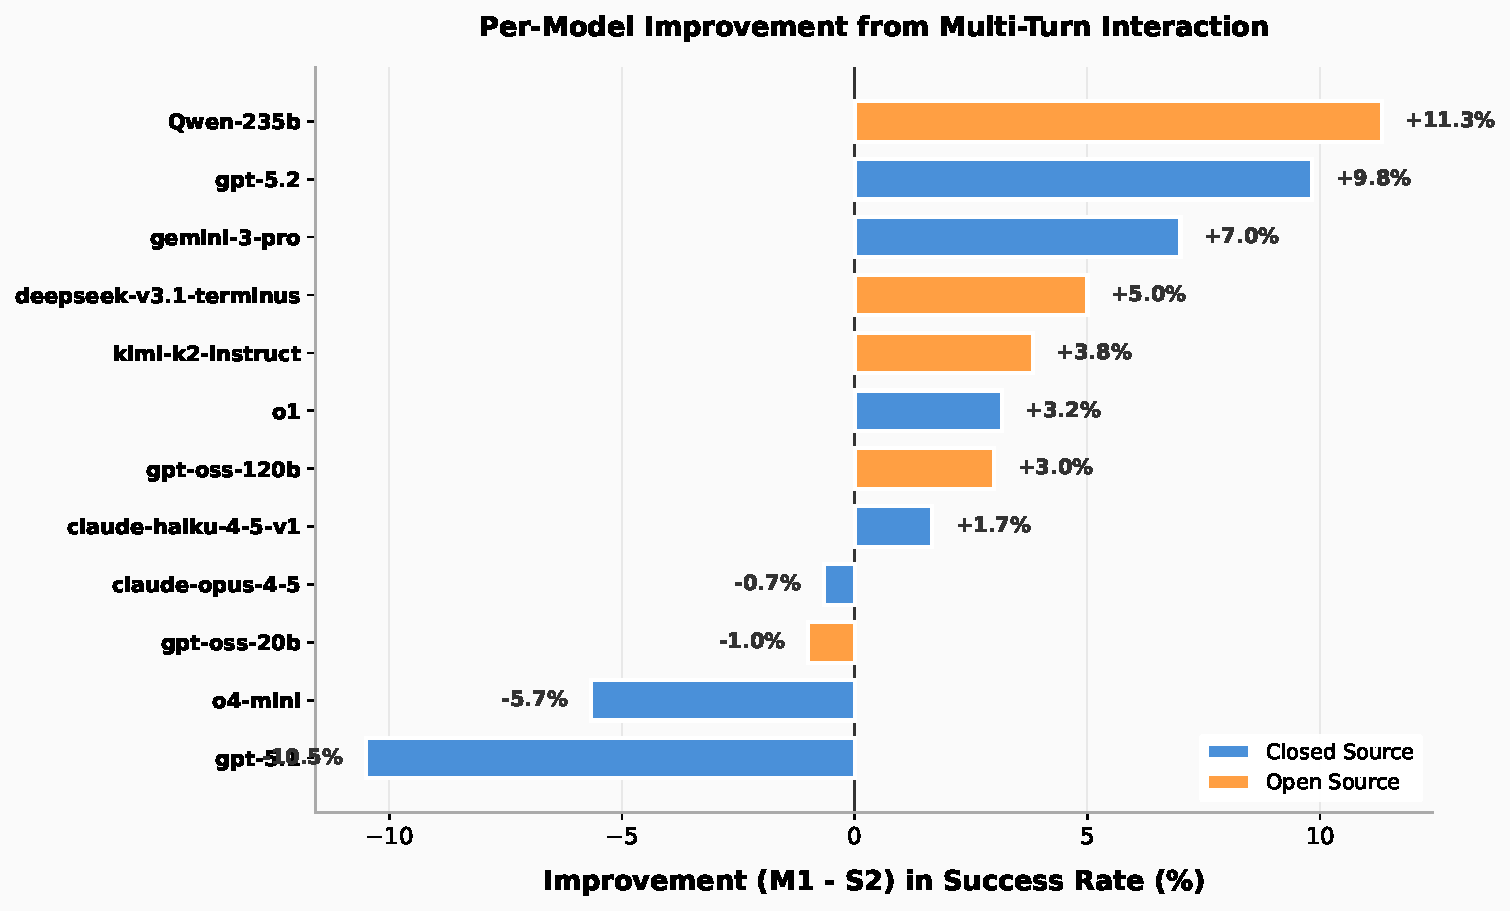
\includegraphics[width=0.45\textwidth]{assets/figures/multiturn_per_model.pdf}
        \caption{Enabling multi-turn interaction with the environment improves task performance.}
        \label{fig:multiturnvssingle}
    \end{figure}
}

\def\visualfeedbackcomp#1{
    \begin{figure}[#1]
        \centering
        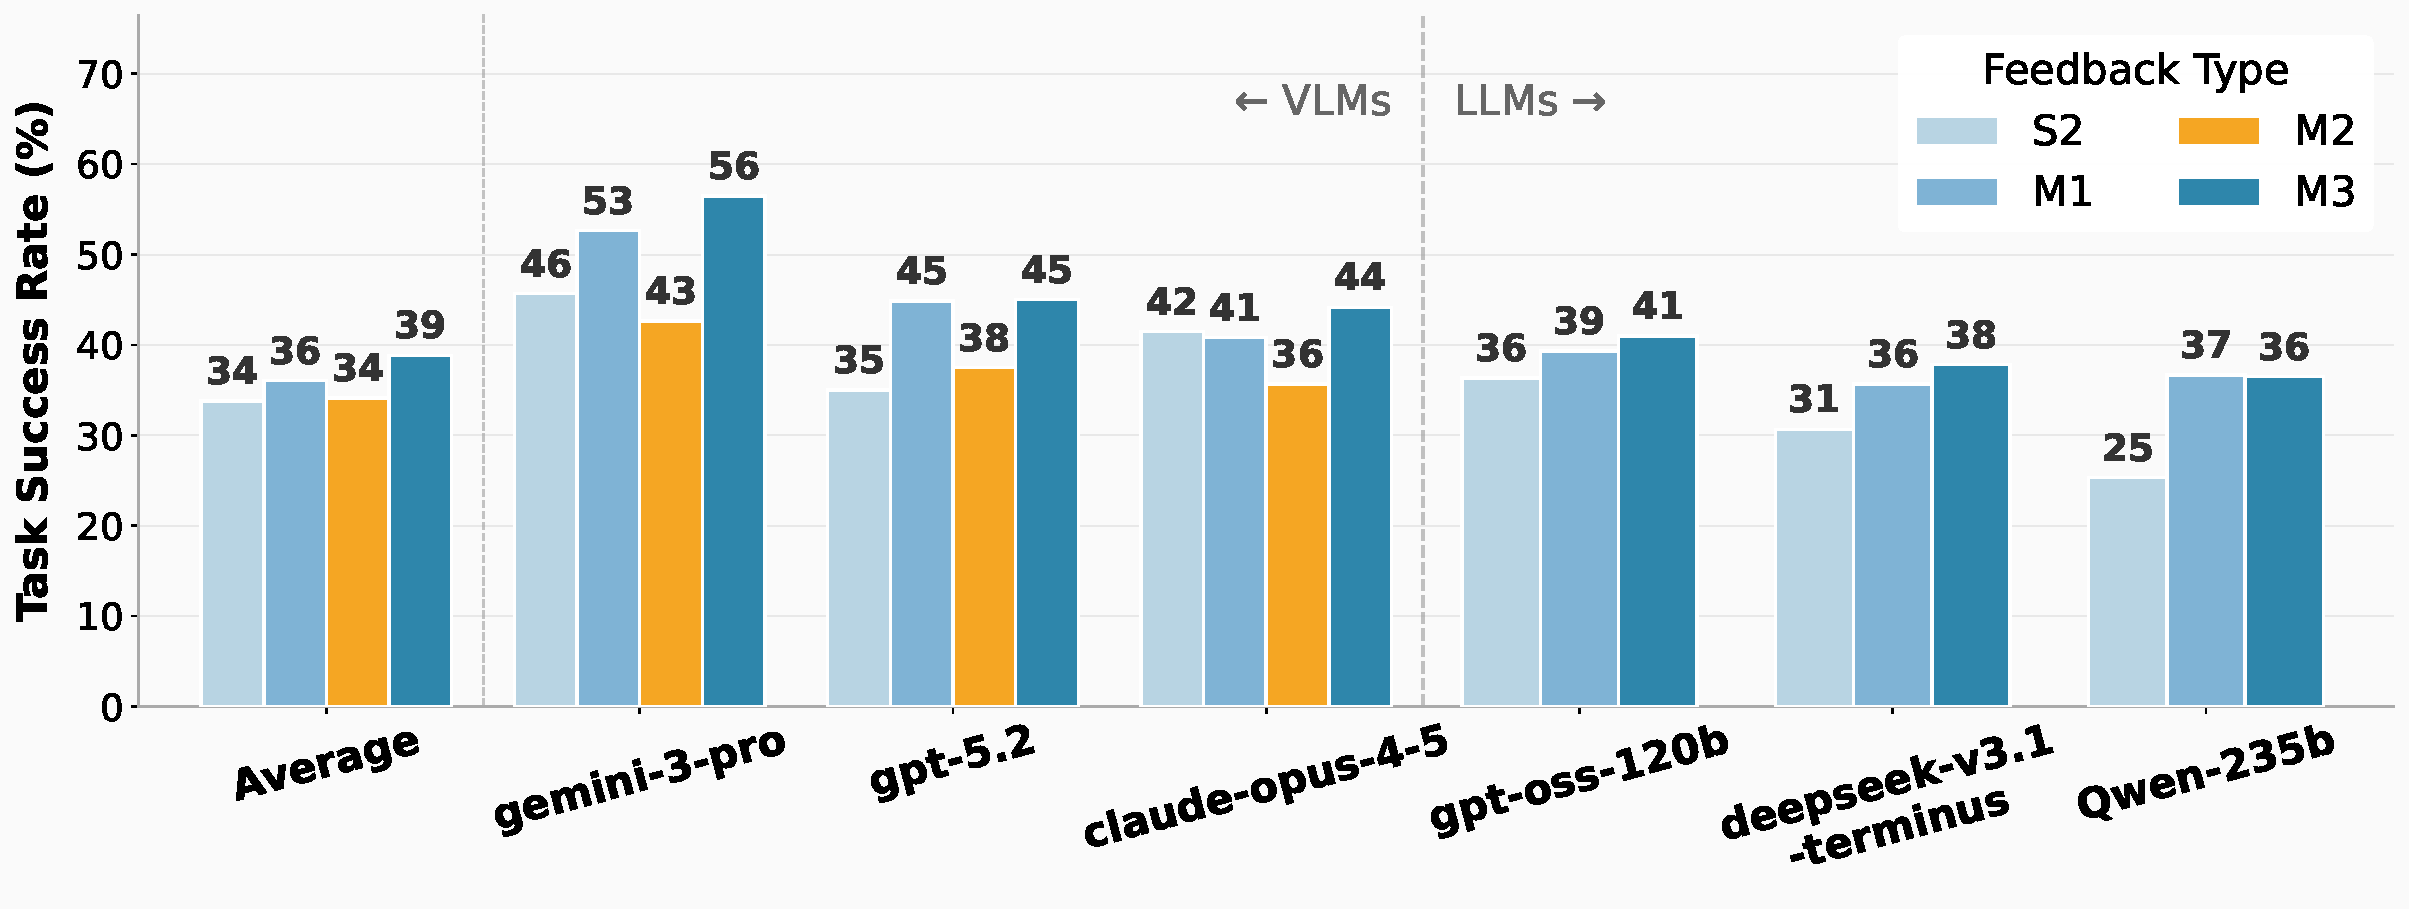
\includegraphics[width=0.45\textwidth]{assets/figures/visual_feedback_comparison.pdf}
        \caption{Comparison of single-turn (S2) and multi-turn tiers (M1-M3) across models. Enabling textual feedback through multi-turn (M1) improves task success rate in most models. Direct multimodal (M2) visual grounding reduced task success rate. We find that visual differencing into text (M3) instead of direct multimodal visual input consistently improves task success rate across both close and open source models. }
        \label{fig:visualfeedbackcomp}
    \end{figure}
}

\def\vdmlvslvsnp#1{
    \begin{figure}[#1]
        \centering
        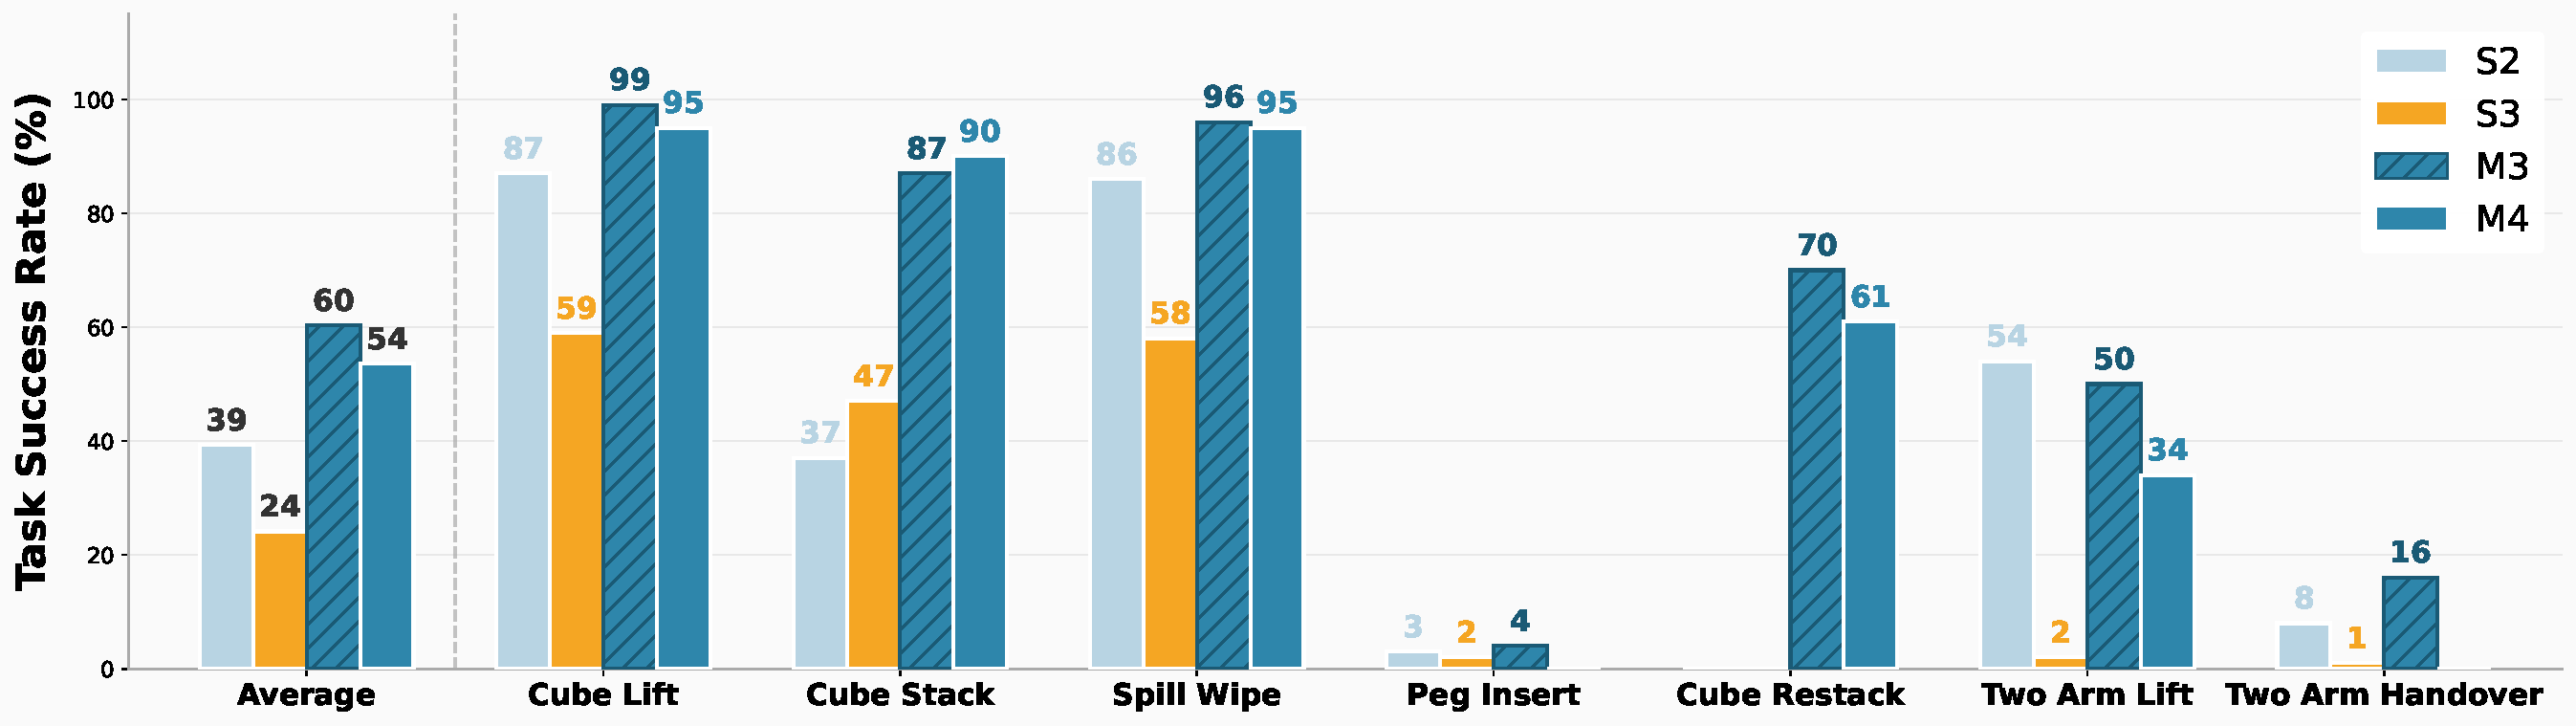
\includegraphics[width=0.45\textwidth]{assets/figures/vdm_l_comparison.pdf}
        \caption{Evaluation of Gemini-3-Pro across four tiers of the benchmark. Multi-turn with visual differencing and low-level API (M4) significantly outperforms both single-turn low-level API (S3), and more notably, single-turn high-level API (S2).}
        \label{fig:vdmlvslvsnp}
    \end{figure}
}

\def\tennisballcasestudy#1{
    \begin{figure*}[#1]
        \centering
        
\includegraphics[width=0.19\textwidth]{assets/figures/case_studies/franka_real_tennis_ball_stack/seq1.png}
        \hfill
        
\includegraphics[width=0.19\textwidth]{assets/figures/case_studies/franka_real_tennis_ball_stack/seq2.png}
        \hfill
        
\includegraphics[width=0.19\textwidth]{assets/figures/case_studies/franka_real_tennis_ball_stack/seq3.png}
        \hfill
        
\includegraphics[width=0.19\textwidth]{assets/figures/case_studies/franka_real_tennis_ball_stack/seq4.png}
        \hfill
        
\includegraphics[width=0.19\textwidth]{assets/figures/case_studies/franka_real_tennis_ball_stack/seq5.png}
        
        \caption{"Stack these as high as you can."}
        \label{fig:tennis_ball_real}
    \end{figure*}
}
\def\restackrealcasestudy#1{
    \begin{figure*}[#1]
        \centering
        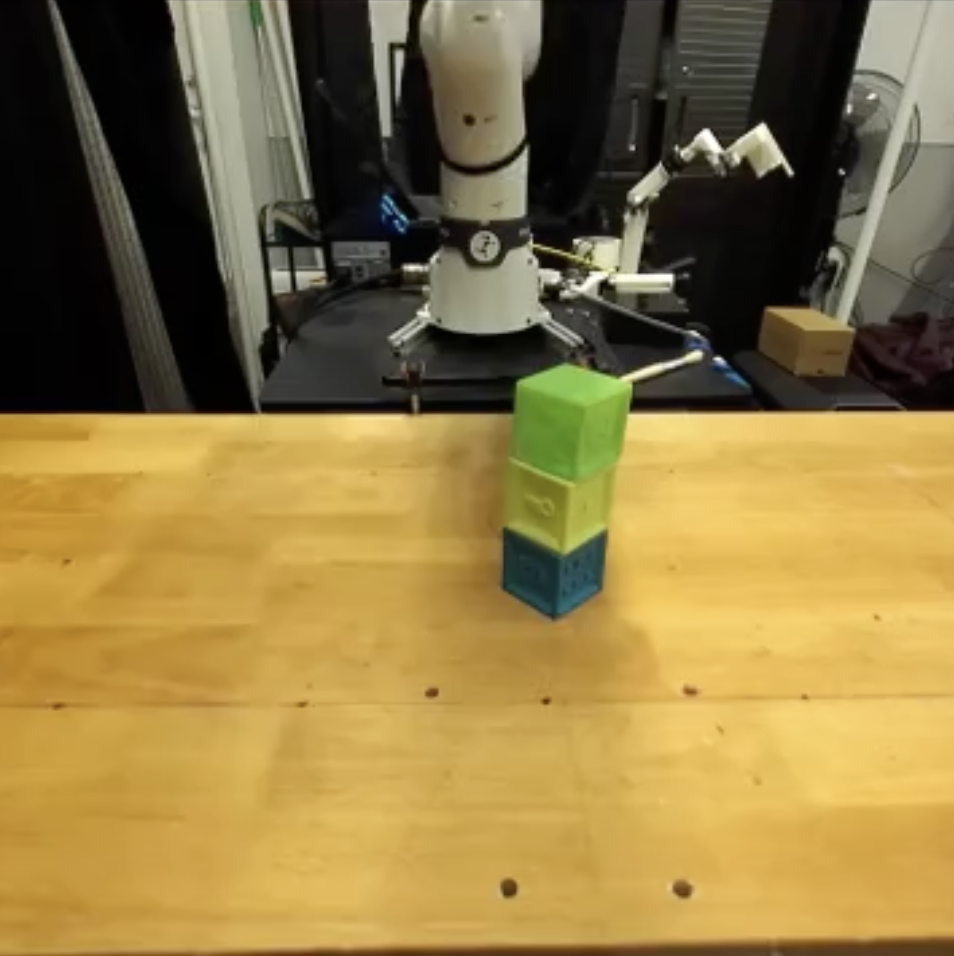
\includegraphics[width=0.19\textwidth]{assets/figures/case_studies/franka_real_restack/seq1.png}
        \hfill
        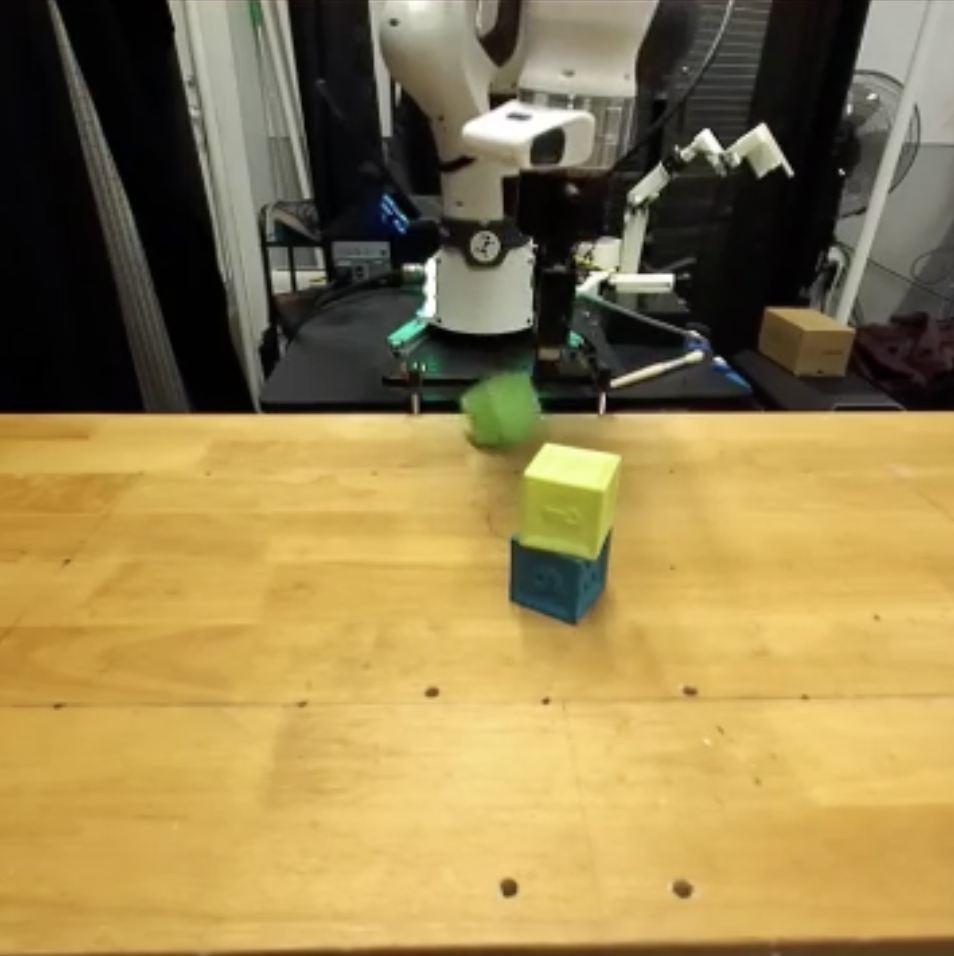
\includegraphics[width=0.19\textwidth]{assets/figures/case_studies/franka_real_restack/seq2.png}
        \hfill
        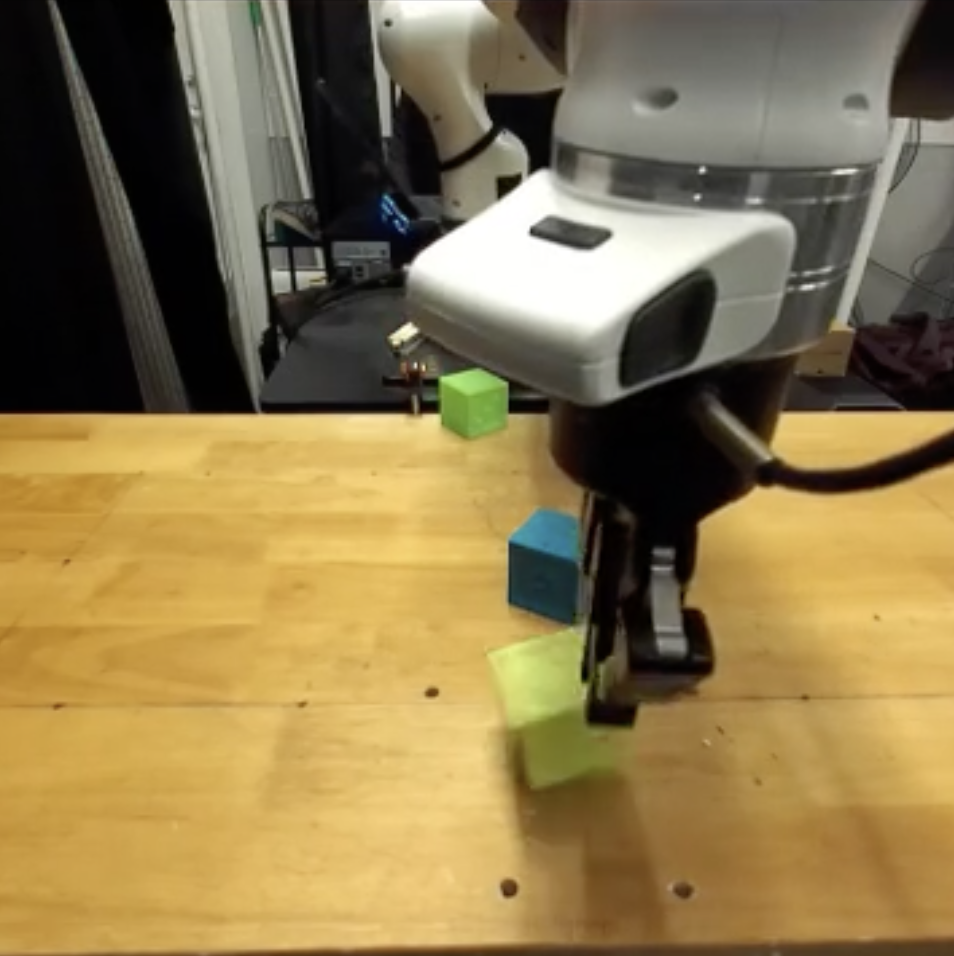
\includegraphics[width=0.19\textwidth]{assets/figures/case_studies/franka_real_restack/seq3.png}
        \hfill
        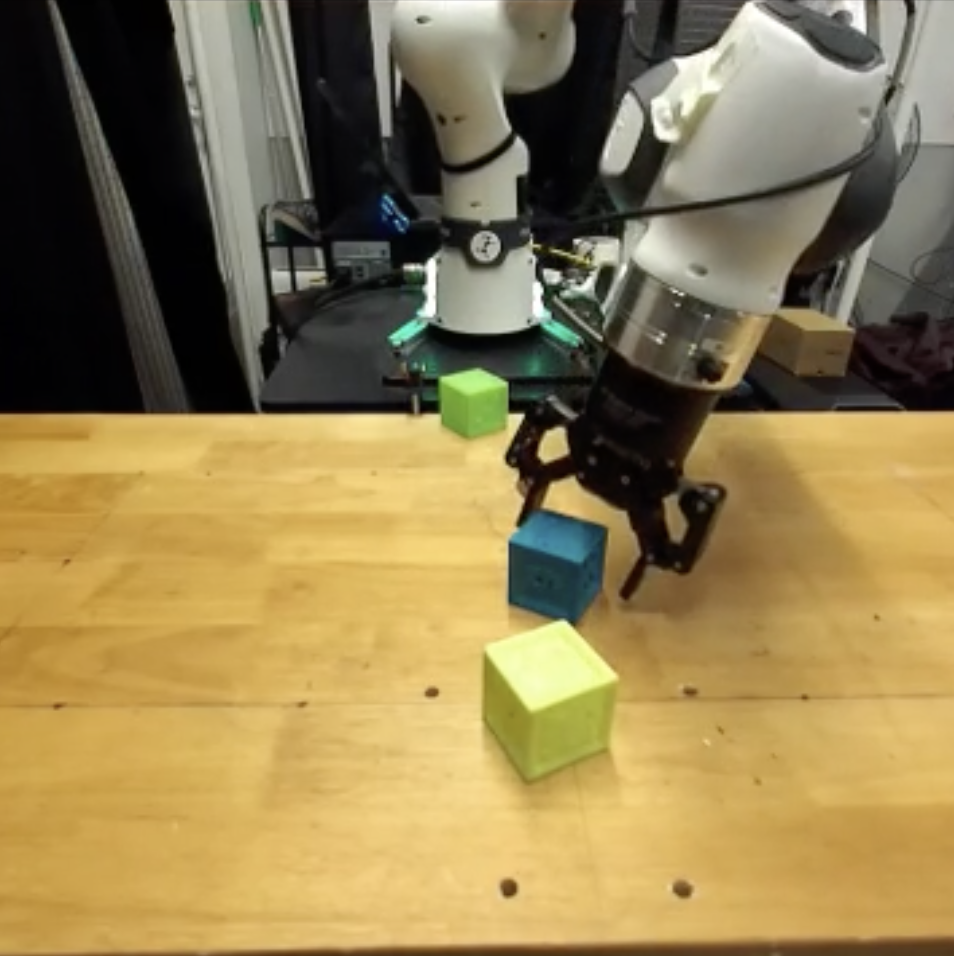
\includegraphics[width=0.19\textwidth]{assets/figures/case_studies/franka_real_restack/seq4.png}
        \hfill
        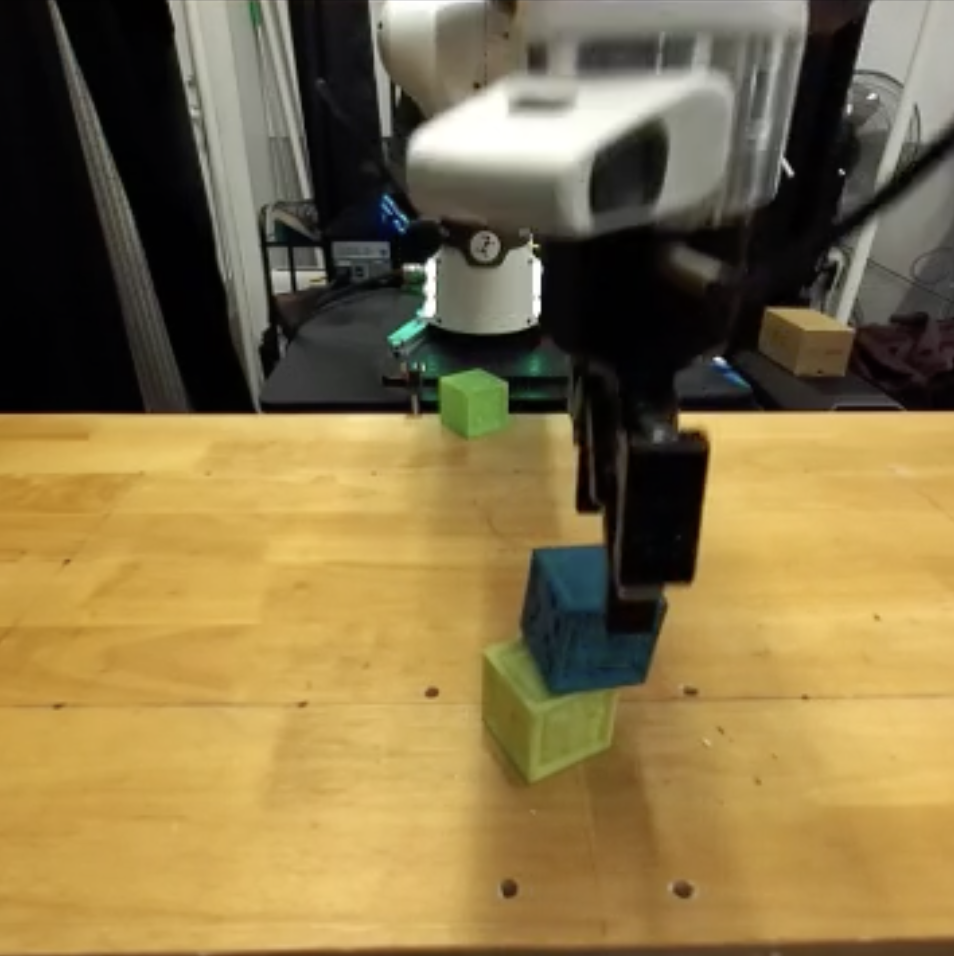
\includegraphics[width=0.19\textwidth]{assets/figures/case_studies/franka_real_restack/seq5.png}
        
        \caption{"Place the blue cube on top of the yellow cube."}
        \label{fig:restack_real}
    \end{figure*}
}

\def\capagentmain#1{
    \begin{figure}[#1]
        \centering
        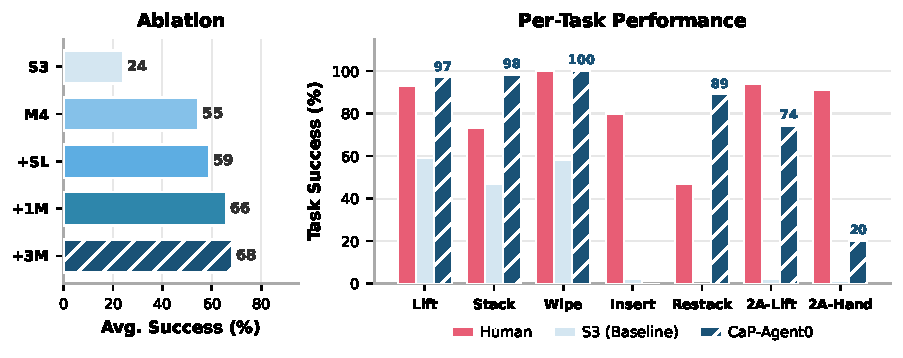
\includegraphics[width=0.45\textwidth]{assets/figures/robomanus_combined.pdf}
        \caption{Ablation for \sysname{}. (Left): Combining VDM (M4), skill library (+SL), and parallel queries (+1M: Gemini-3-Pro, +3M: Gemini-3-Pro, GPT-5.2, and Claude Opus) significantly improves over single-turn setup with low-level API. (Right): On 4 out of 7 \benchname{} tasks, \sysname{} achieves comparable or better success rates than human expert code in a single-turn setting.
        }
        \label{fig:capagentmain}
    \end{figure}
    \vspace{-5.0pt}
}

\def\prepostrlreal#1{
    \begin{figure}[#1]
        \centering
        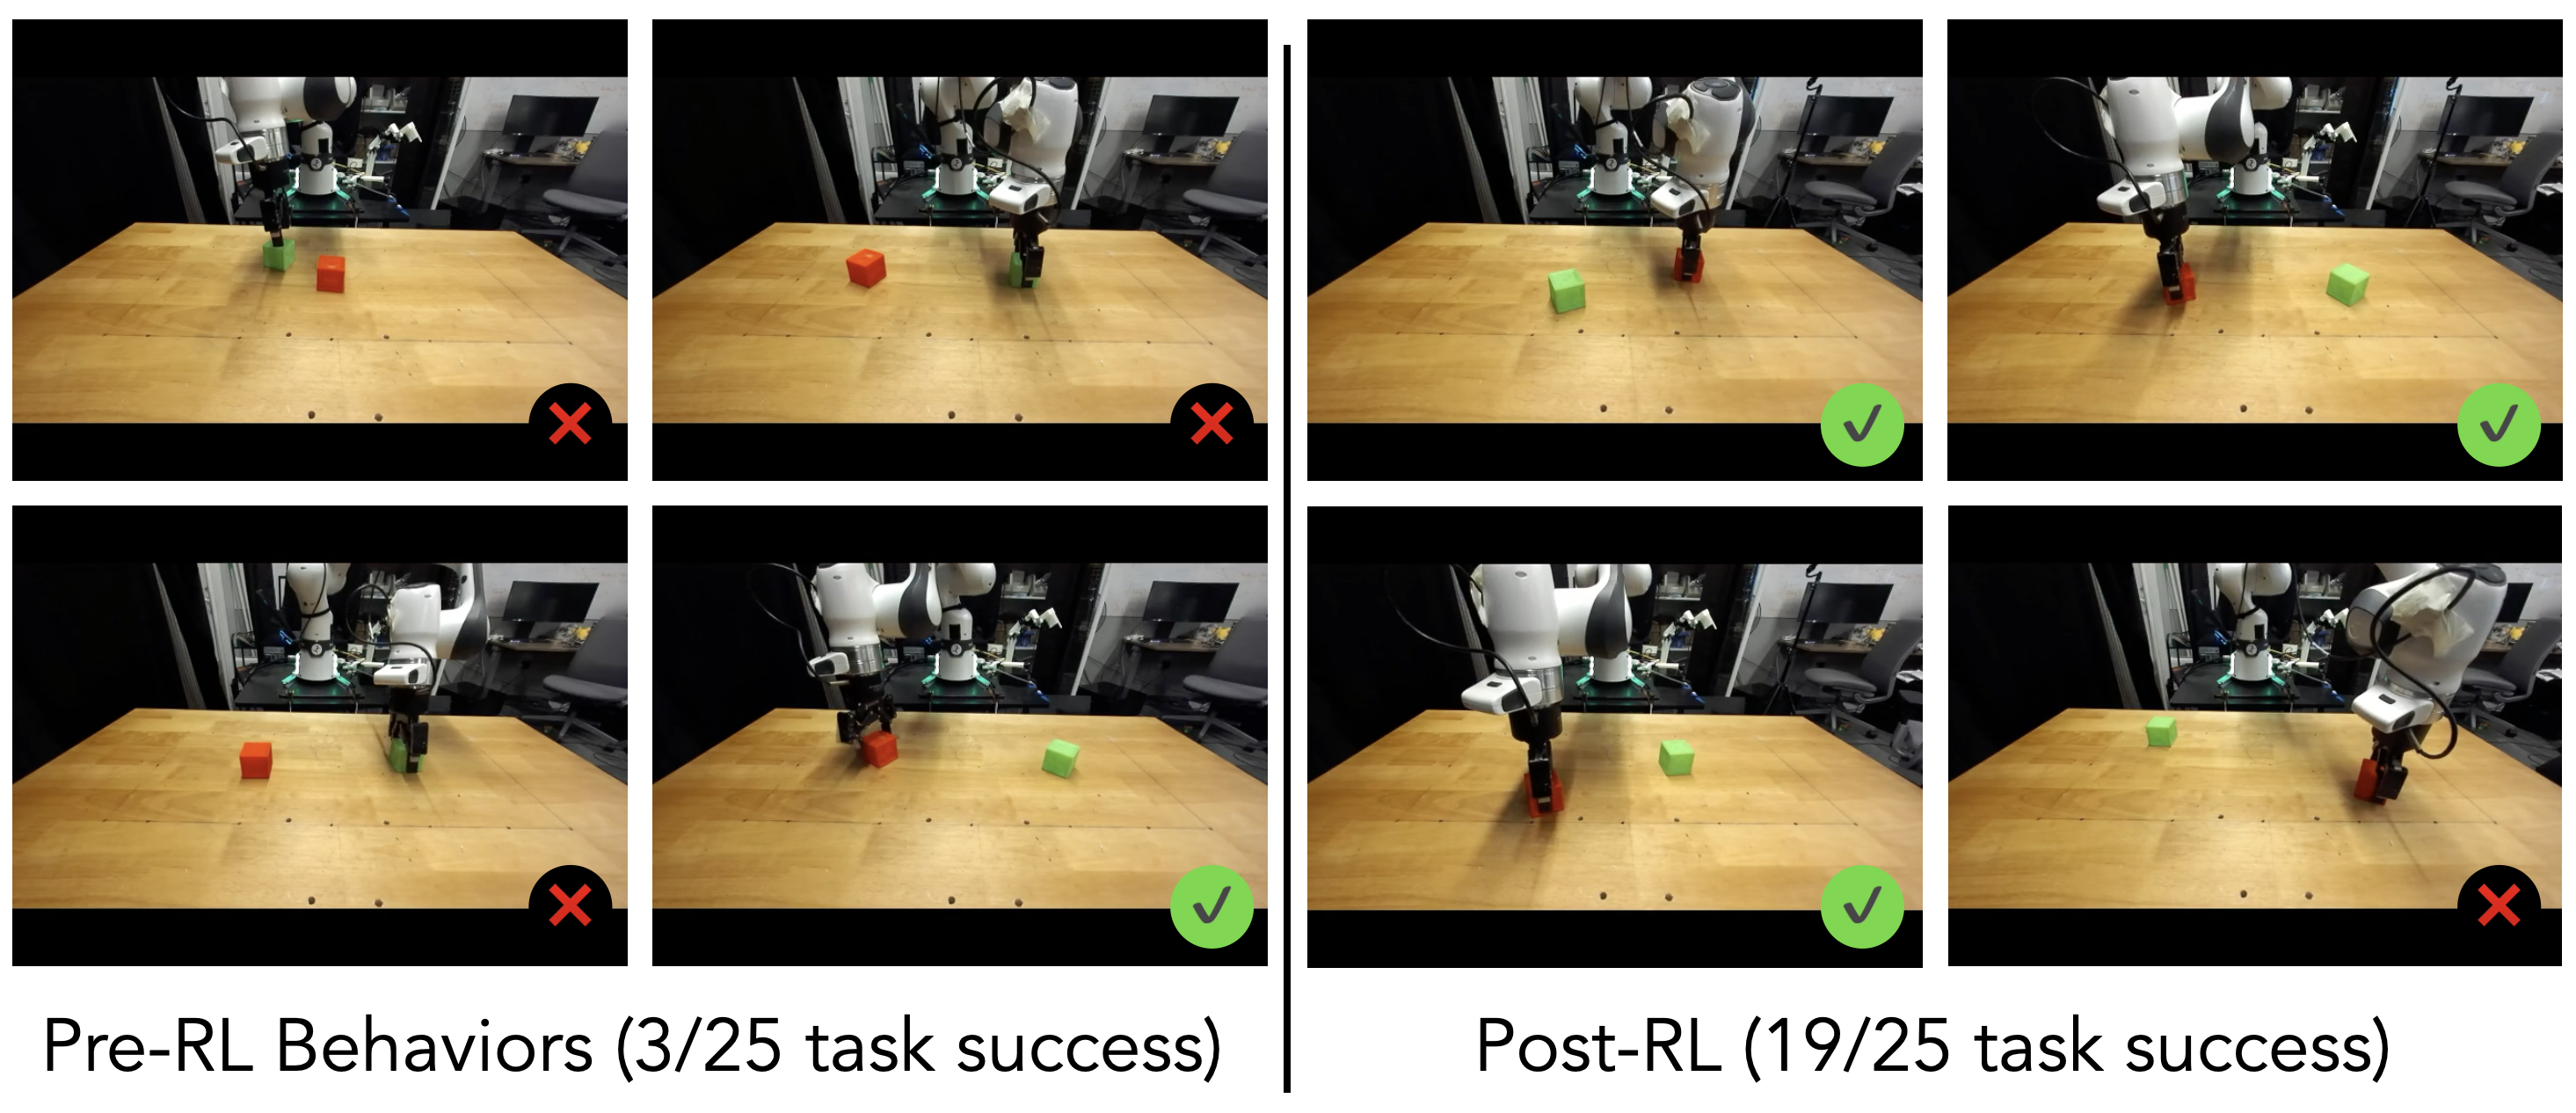
\includegraphics[width=\textwidth]{assets/figures/pre-post-RL-real-eval.png}
        \caption{CaP-RL Finetuned Qwen-2.5-Coder-7B-Instruct deployed on the real task \textit{put the red cube on the green cube}. Human Oracle code gets 21/25 task successes in real. Prior to reinforcement learning, we see behaviors such as grasp approaches on the green cube as the first action, rather than a more sensible approach on the red cube first.}
        \label{fig:RL_real_franka}
    \end{figure}
}

\def\postrlgeneralization#1{
    \begin{figure}[#1]
        \centering
        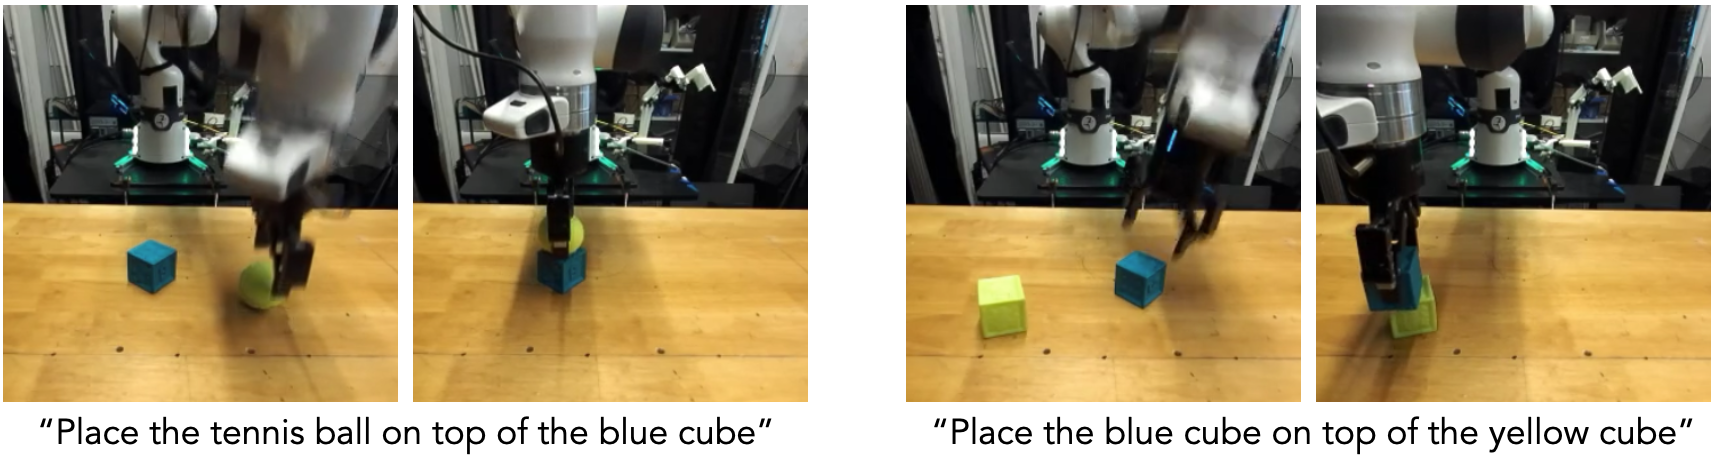
\includegraphics[width=\textwidth]{assets/figures/postRLgeneralization.png}
        \caption{CaP-RL Finetuned Qwen-2.5-Coder-7B-Instruct successfully deployed on similar task variants. Demonstrates that base model is still capable of instruction following.}
        \label{fig:postRLgeneral}
    \end{figure}
}

\def\fullbenchtable#1{
    \begin{figure}[#1]
        \centering
        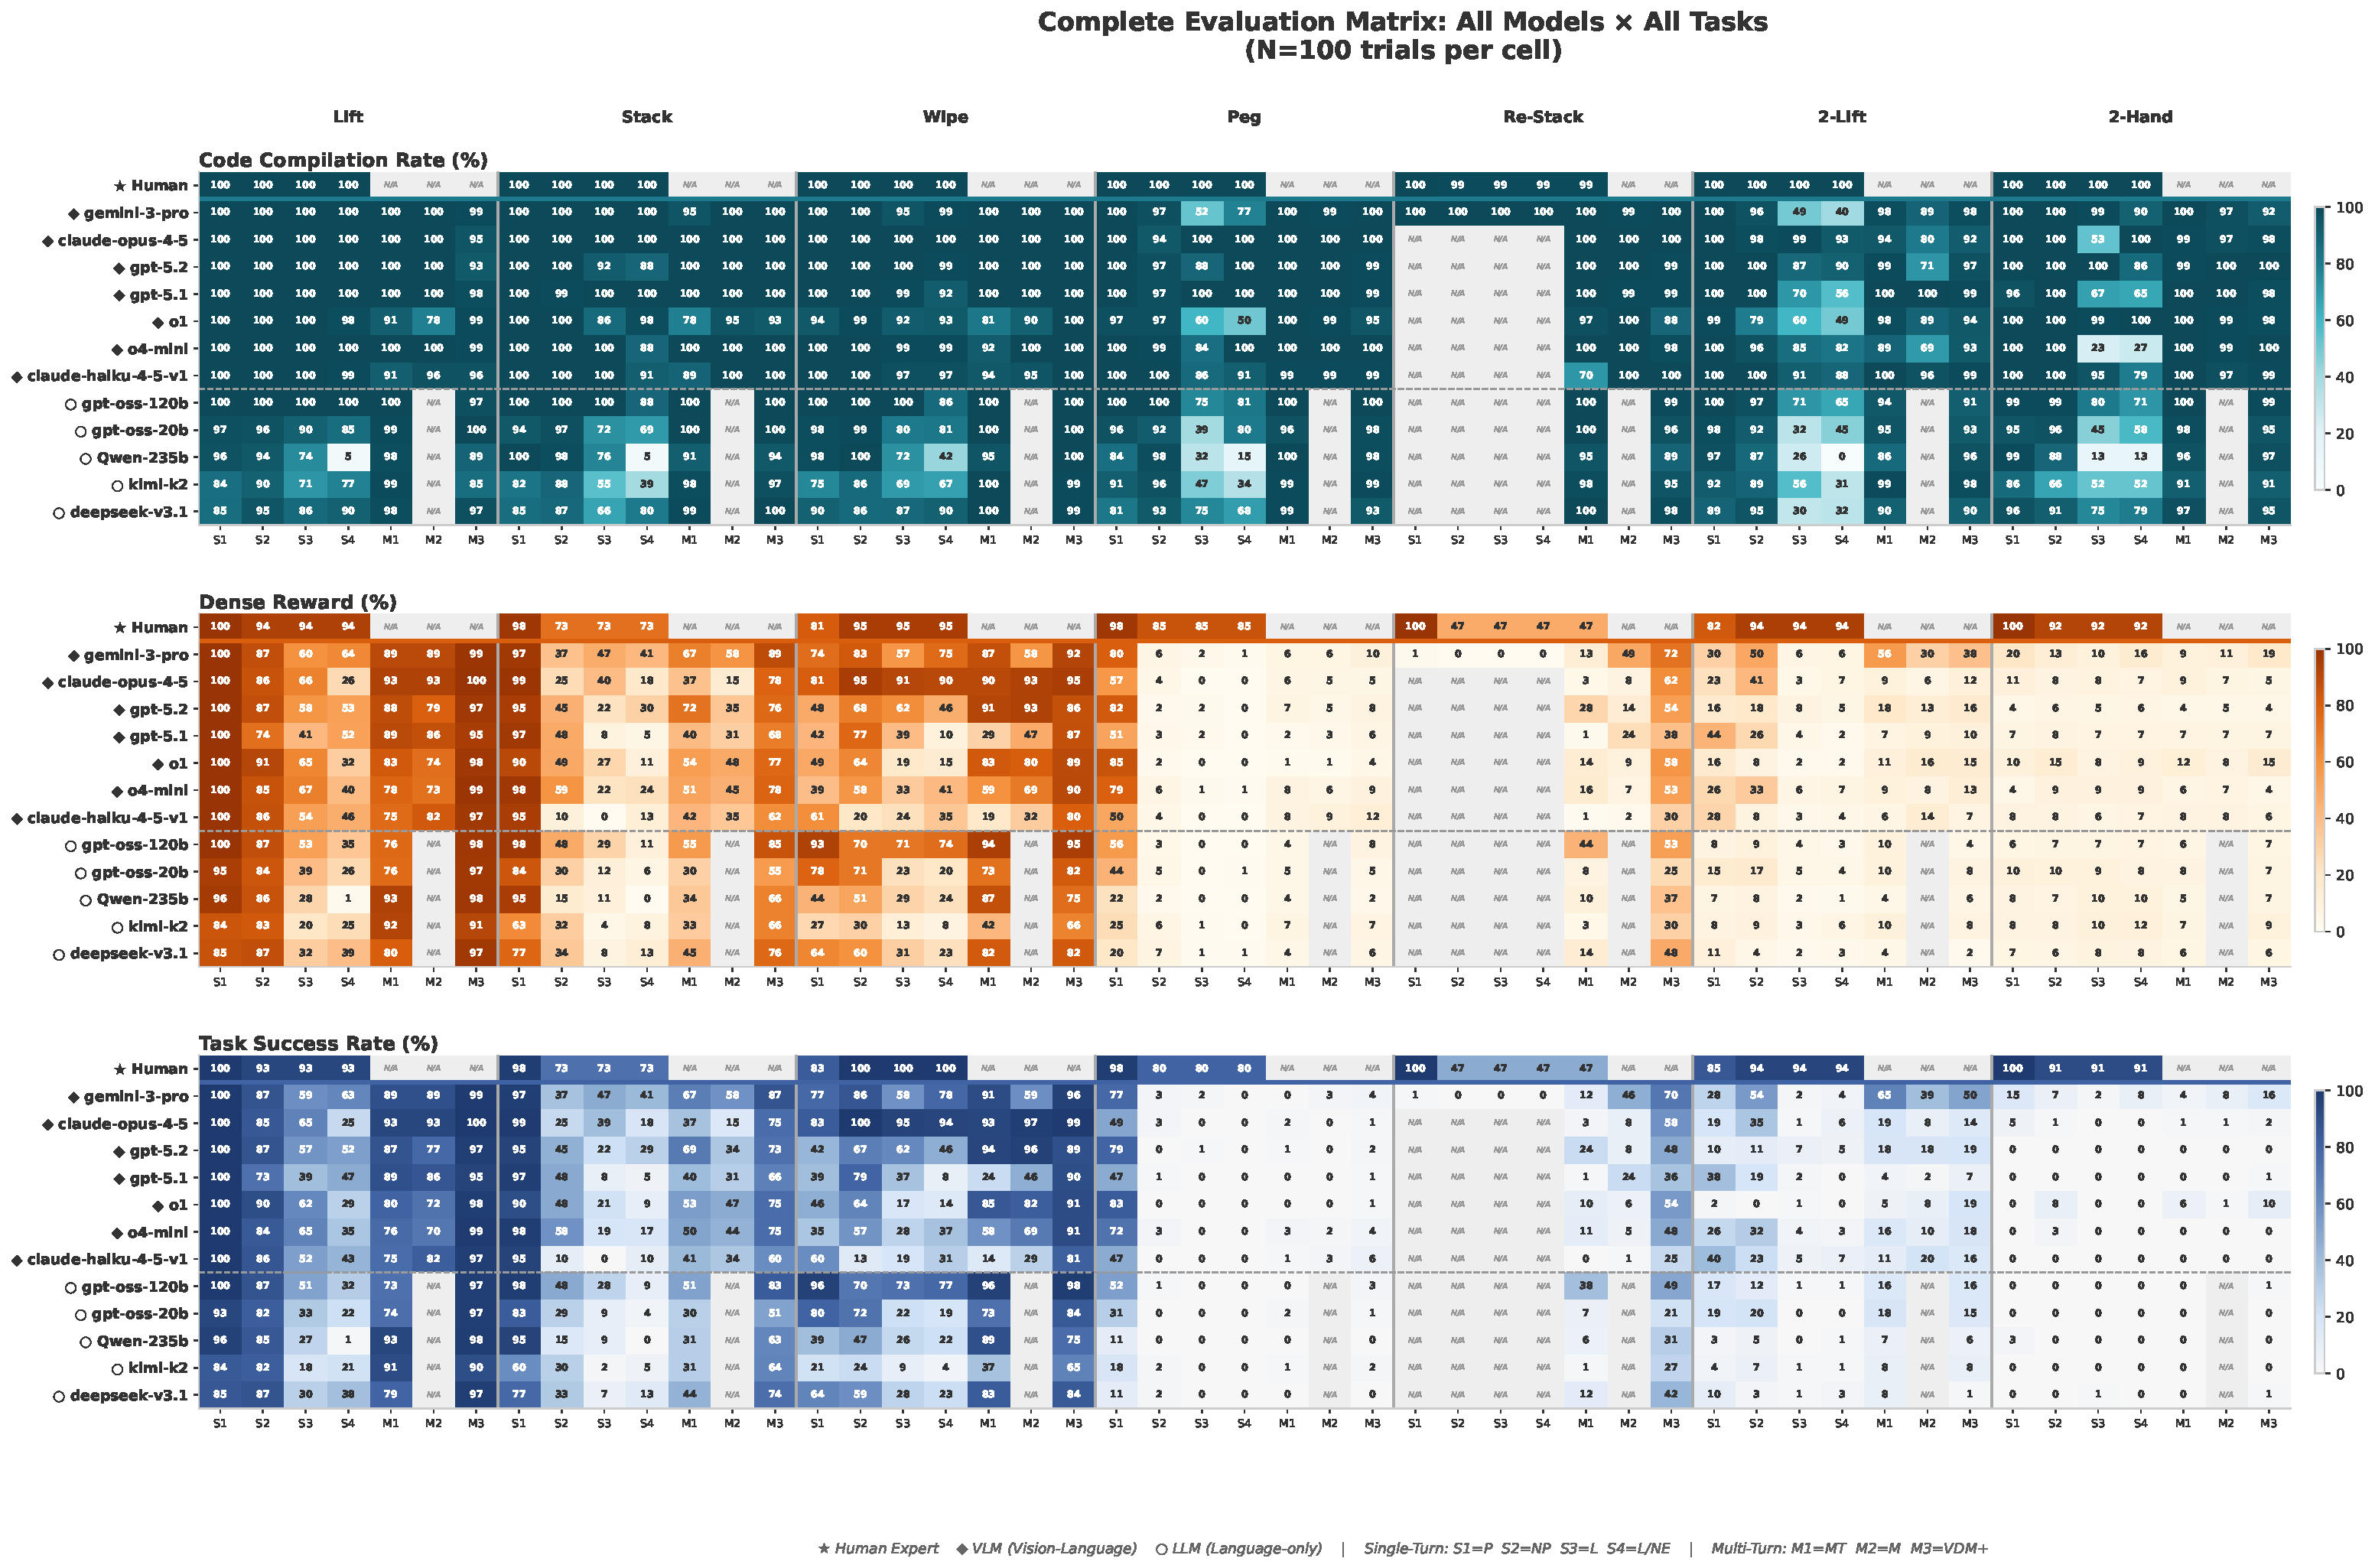
\includegraphics[width=\textwidth]{assets/figures/main_results_heatmap.pdf}
        \caption{Full \benchname{} results. From top to bottom are code compilation success rates, average task reward, and average task success rate. Note that for \texttt{Re-Stack}, with a simple task prompt, without visual input, we do not observe model writing code to first check the initial condition and then perform the task, resulting in failures. Therefore, we only evaluatd all models for the multi-turn setup.}
        \label{fig:fullbenchtable}
    \end{figure}
}
